\documentclass[czech]{beamer}

\usepackage{mathptmx}

\usepackage[utf8]{inputenc}
\usepackage[czech]{babel}
\usepackage{color}

\usepackage{amsmath}
\usepackage{amsfonts}
\usepackage{amssymb}

\usepackage{mathtools}
\usepackage{floatflt}
\usepackage{graphicx}

\usepackage{tikz}
\usepackage{pgf}

\usepackage{stmaryrd}

\usepackage{colortbl}


\usetikzlibrary{arrows,snakes}

\newcommand{\bomega}{\ensuremath{\mathbf{\Omega}}}
\newcommand{\tinydot}{\mbox{\tiny{\textbullet}}}
\newcommand{\keff}{\ensuremath{k_{\mathrm{eff}}}}
\newcommand{\br}{\ensuremath{\mathbf{r}}}
\newcommand{\bn}{\ensuremath{\mathbf{n}}}
\newcommand{\bj}{\ensuremath{\mathbf{j}}}
\newcommand{\bJ}{\ensuremath{\mathbf{J}}}

\newcommand{\RR}[1][]{\mathbb{R}^{#1}}

\newcommand{\EE}{\mathcal{E}}
\renewcommand{\SS}{\ensuremath{\mathcal{S}}}
\newcommand{\VV}{\mathcal{V}}

\newcommand{\bnd}{\ensuremath{\partial\VV}}
\newcommand{\pX}[1][]{\partial X^{#1}}
\newcommand{\pV}[1][]{\partial \VV}
\newcommand{\pVh}[1][]{\partial \VV_h}
\newcommand{\pVn}[1][]{\partial \VV_{0}}

\newcommand{\pd}[3][]{\ensuremath{\frac{\partial^{#1}#2}{\partial #3^{#1}}}}
\newcommand{\der}[3][]{\ensuremath{\frac{\mathrm{d}^{#1}{#2}}{\mathrm{d} {#3}^{#1}}}}

\newcommand{\abs}[1]{\ensuremath{\left\vert#1\right\vert}}
\newcommand{\norm}[2][]{\ensuremath{\lvert\lvert#2\rvert\rvert_{#1}}}

\newcommand{\Rabullet}{\ensuremath{\structure{\Rightarrow}}}
\newcommand{\ra}{\ensuremath{\!\rightarrow\!}}
\newcommand{\la}{\ensuremath{\!\leftarrow\!}}

\newcommand{\eint}[1]{\ensuremath{\int_{0}^{\infty}#1\,\d{E}}}
\newcommand{\Eint}[2][\EE]{\ensuremath{\int_{#1}{#2}\,\d{E}}}
\newcommand{\vint}[1]{\ensuremath{\int_{\VV}{#1}\,\d{\br}}}
\newcommand{\Vint}[2][\VV]{\ensuremath{\int_{#1}{#2}\,\d{\br}}}
\newcommand{\aint}[1]{\ensuremath{\int_{4\pi}{#1}\,\d{\bomega}}}
\newcommand{\Aint}[2][\SS]{\ensuremath{\int_{#1}{#2}\,\d{\bomega}}}
\newcommand{\eintp}[1]{\ensuremath{\int_{0}^{\infty}#1\,\d{E'}}}
\newcommand{\vintp}[1]{\ensuremath{\int_{\VV}{#1}\,\d{\br'}}}
\newcommand{\aintp}[1]{\ensuremath{\int_{4\pi}{#1}\,\d{\bomega'}}}
\newcommand{\bndint}[2][]{\displaystyle\int_{#2}\db{x#1}}
\newcommand{\db}[1]{\ensuremath{\mathrm{d_b}#1\,}}
\renewcommand{\d}[1]{\ensuremath{\mathrm{d}#1\,}}

\newcommand{\fl}{\ensuremath{\phi}}
\newcommand{\flux}{\ensuremath{\phi}}
\newcommand{\afl}{\ensuremath{\psi}}
\newcommand{\angflux}{\ensuremath{\psi}}
\newcommand{\angfluxin}{\angflux_{\mathrm{in}}}

\newcommand{\MM}{\ensuremath{\mathbf{M}}}
\newcommand{\FF}{\ensuremath{\mathbf{F}}}
\newcommand{\QQ}{\ensuremath{\mathbf{Q}}}

\newcommand{\llop}{\ensuremath{\mathbf{L}}}
\newcommand{\hhop}[1][]{\ensuremath{\mathbf{H}}_{#1}}
\newcommand{\ffop}{\ensuremath{\mathbf{F}}}
\newcommand{\vangflux}{\ensuremath{\boldsymbol{\psi}}}
\newcommand{\valbedo}{\ensuremath{\boldsymbol{\beta}}}

\newcommand{\vv}{\ensuremath{\mathbf{v}}}

\newcommand{\Lp}[2][]{L_{#1}^{#2}}
\newcommand{\Wp}[2][]{W_{#1}^{#2}}
\newcommand{\Id}{I}

\newenvironment{myitemize}{
\begin{itemize}\vspace*{.5em}
  \setlength{\itemsep}{1em}
}{\end{itemize}}

\newcommand{\sumg}{\sum_{\makebox[0pt]{${\scriptscriptstyle{g'\neq g}}$}}}
\newcommand{\sumr}{\sum_{\scriptscriptstyle{R=f,s}}}

\newcommand{\Sgmr}{\Sigma_{\rightarrow}}
\newcommand{\Sgml}{\Sigma_{\leftarrow}}

\newcommand{\polar}{\vartheta}
\newcommand{\azimuthal}{\varphi}
\renewcommand{\P}[1]{P_{#1}}
\newcommand{\suma}[3][l]{\sum_{#1=#2}^{#3}}
\newcommand{\muint}[1][]{\int_{-1}^{1}\d{\mu#1}}
\newcommand{\muav}{\overline{\mu}_0}
\newcommand{\sint}{\sin \polar}
\newcommand{\sinp}{\sin \azimuthal}
\newcommand{\cost}{\cos \polar}
\newcommand{\cosp}{\cos \azimuthal}
\newcommand{\lvec}[1]{\big[#1\big]}
\newcommand{\lvect}[1]{\big[#1\big]^T}


\newcommand{\Y}[2]{Y_{#1}^{#2}}
\newcommand{\Yc}[2]{\bar{Y}_{#1}^{#2}}
\newcommand{\kron}[2]{\delta_{#1#2}}
\newcommand{\angmomgen}[2]{\ensuremath{\phi_{#1#2}}}


\definecolor{dkblue}{named}{blue}
\definecolor{dkgreen}{rgb}{0,0.4,0}
\definecolor{dkred}{rgb}{0.4,0,0}
\definecolor{dkgrey}{rgb}{0.4,0.4,0.4}
\definecolor{ltgrey}{rgb}{0.6,0.6,0.6}
\colorlet{matA}{black!15}
\colorlet{matB}{red!30}
\colorlet{matC}{green!30}
\colorlet{matAdk}{black!80}
\colorlet{matBdk}{red!70}
\colorlet{matCdk}{green!70}

\newcommand{\tocrule}{\hspace{.0342\textwidth}\color{structure}\rule{.618\textwidth}{.25mm}}

\newlength\celldim \newlength\fontheight \newlength\extraheight
\setlength\celldim{2em}
\settoheight\fontheight{A}
\setlength\extraheight{\celldim - \fontheight}

\newcolumntype{A}{ >{\centering \columncolor{matA}} p{.2\linewidth} <{\rule[-.5\extraheight]{0pt}{\extraheight+\fontheight}}}
\newcolumntype{B}{ >{\centering \columncolor{matB}} p{.2\linewidth} <{\rule[-.5\extraheight]{0pt}{\extraheight+\fontheight}}}
\newcolumntype{C}{ >{\centering \columncolor{matC}} p{.2\linewidth} <{\rule[-.5\extraheight]{0pt}{\extraheight+\fontheight}}}
\newcommand{\nl}{\tabularnewline\hline}

\let\Oldpart\part
\newcommand{\parttitle}{}
\renewcommand{\part}[1]{\Oldpart{#1}\renewcommand{\parttitle}{#1}}

\def\shorten#1#2{\bgroup
\addtolength\abovedisplayshortskip{#1}
\addtolength\abovedisplayskip{#1}
\addtolength\belowdisplayshortskip{#2}
\addtolength\belowdisplayskip{#2}
}
\def\lengthen{\egroup}


%\renewcommand{\bfdefault}{sb}



%%%%%%%%%%%%%%%%%%%%%%%%%%%%%% User specified LaTeX commands.
%\usetheme{Warsaw}
\usetheme{Boadilla}
% or ...

\usecolortheme{orchid}
\setbeamertemplate{footline}[text line]{} % makes the footer EMPTY

% \setbeamercovered{transparent}

\AtBeginSection[]{%
	\addtocounter{framenumber}{-1}
  	\begin{frame}[t]
   	\centering\frametitle{\parttitle}
   	\tableofcontents[currentsection, hideothersubsections]
	\end{frame}
}

\begin{document}

\everymath{\displaystyle}
%\beamerdefaultoverlayspecification{<+->}

% For every picture that defines or uses external nodes, you'll have to
% apply the 'remember picture' style. To avoid some typing, we'll apply
% the style to all pictures.
\tikzstyle{every picture}+=[remember picture]
\tikzstyle{na} = [baseline=-.5ex]


\title{Deterministické řešení transportní rovnice neutronů}
\author{Milan Hanuš,\\[.2em]
{\small\textcolor{ltgrey}{KMA, FAV ZČU Plzeň}}}
\date[MORF 1]{{Transportní rovnice v reaktorové fyzice}\\[.2em]
{\small\textcolor{ltgrey}{15. 4. 2009}}}

\begin{frame}[label=s0]
	\titlepage
\end{frame}

\begin{frame}[allowframebreak]
%	\frametitle{Přehled}
 	  \tableofcontents
\end{frame}

%\part{Transportní rovnice neutronů}
%
  \section{Předpoklady a definice}
    \begin{frame}
  \frametitle{Základní předpoklady}
  
  \begin{itemize}
  	\item Neutrony lze popsat jako bodové objekty, ovlivněné pouze jadernými silami
  	\begin{itemize}
  		\item[\Rabullet] pohyb neutronů po přímých drahách
  		\item[\Rabullet] interakce s okolními atomy vede k záchytu či změně směru anebo rychlosti neutronu
  	\end{itemize}
  	\item Vzájemné interakce mezi neutrony jsou zanedbatelné
  	\item Izotropní prostředí, atomy sféricky symetrické
  	\begin{itemize}
  		\item samotný rozptyl a pohyb neutronů však může být anizotropní
  	\end{itemize}
  	\item Stacionární rozložení atomů (zanedbáváme tepelný pohyb)
  \end{itemize}

  \uncover<2->{
    \alert{Pohyb neutronů prostředím lze popsat lineární Boltzmannovou rovnicí}
    \begin{center}
    	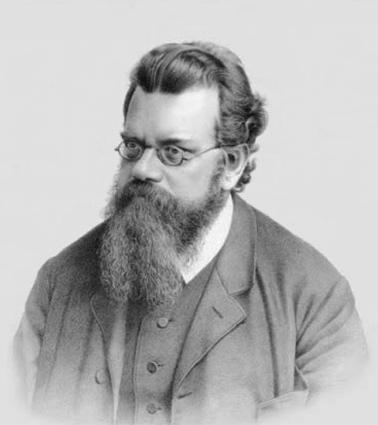
\includegraphics[scale=0.30]{obr/Boltzmann.jpg}
    \end{center}
  }
  
\end{frame}

\begin{frame}[t]
  \frametitle{Stavový prostor}
 
  $$
    X = \VV \times \EE \times \SS \equiv \{x = (\br,E,\bomega):\ \br\in \VV, E \in \EE, \bomega\in \SS\}
  $$
  
  \begin{center}
	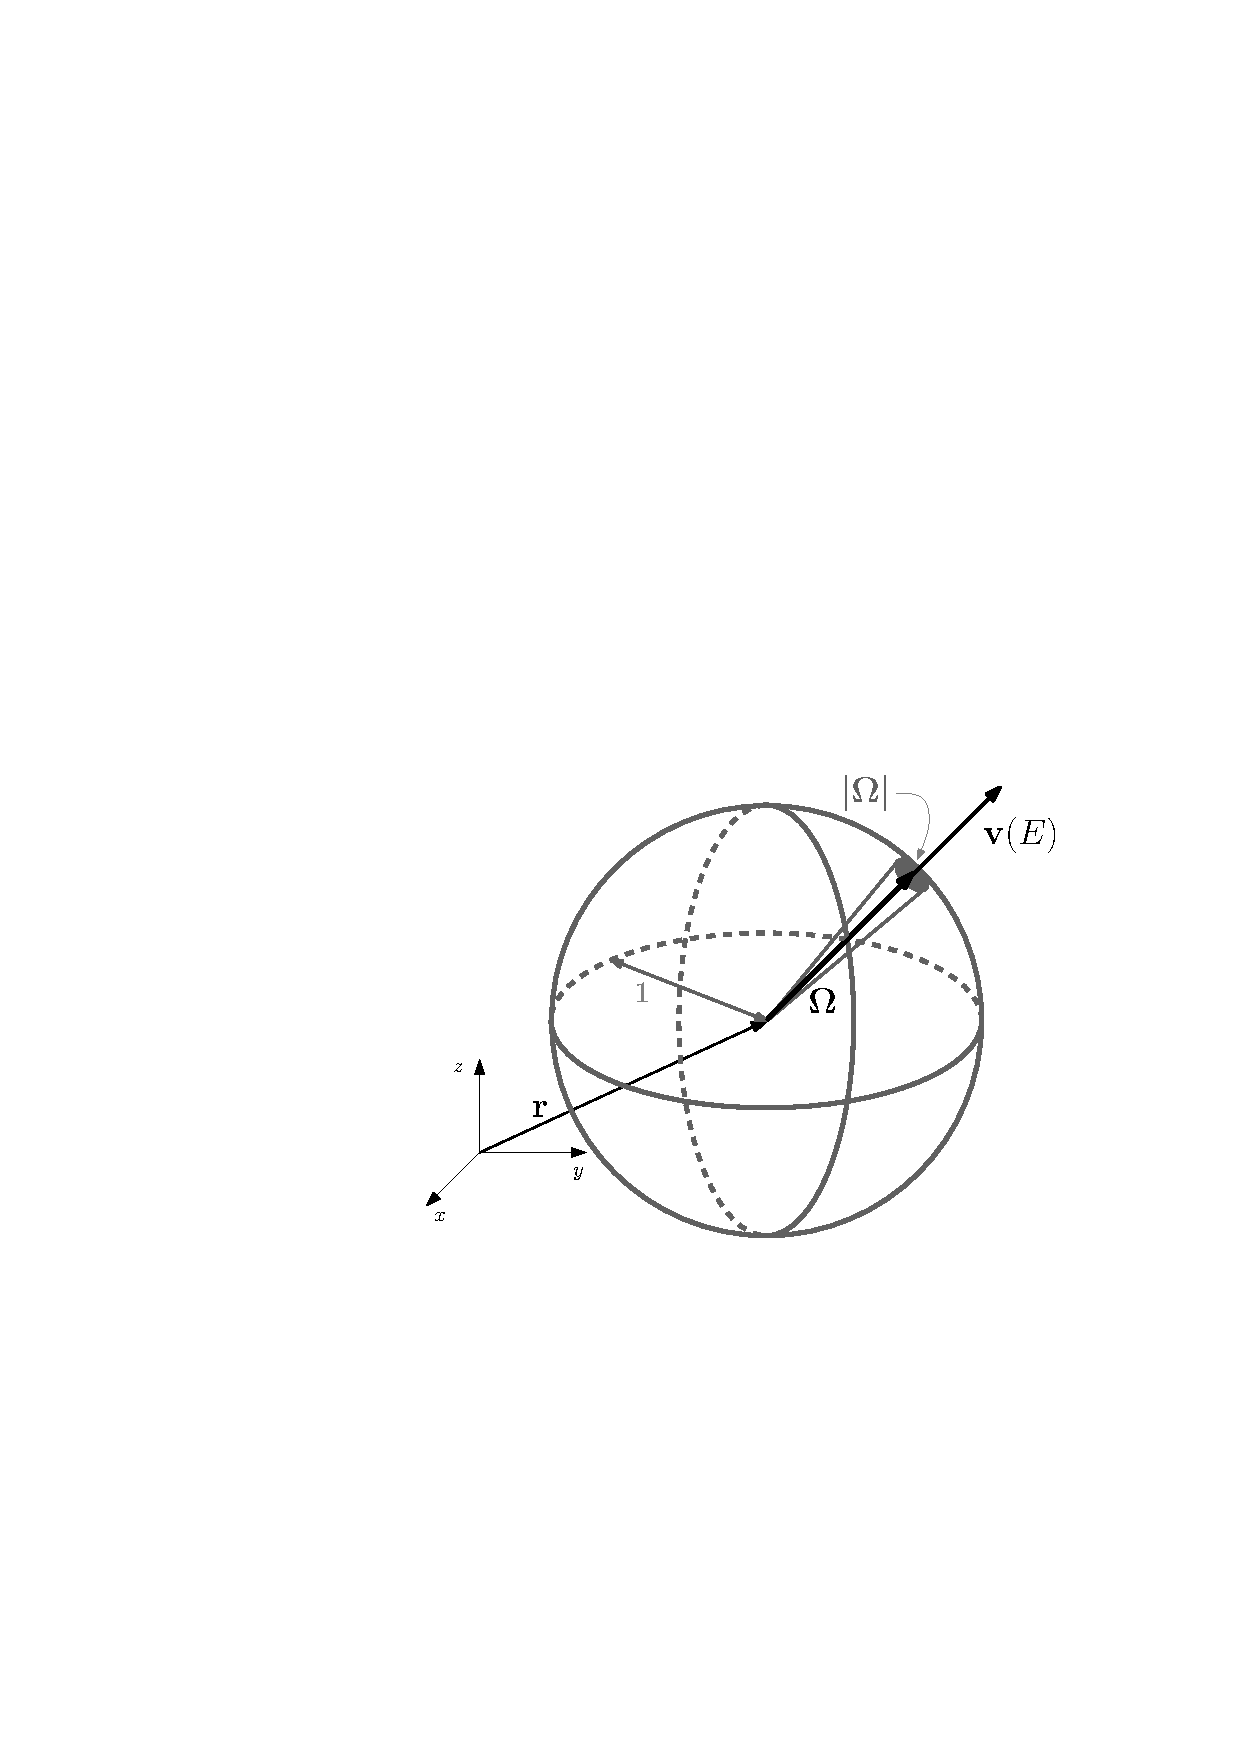
\includegraphics[scale=0.70]{obr/stavovy_prostor}\\[1em]
	\alert{6 dimenzí}
  \end{center}

\end{frame}

\begin{frame}[t]
  \frametitle{Stavový prostor}
  \framesubtitle{Poloha}
 
  $$
    X = \VV \times \EE \times \SS \equiv \{x = (\alert\br,E,\bomega):\ \alert{\br\in \VV}, E \in \EE, \bomega\in \SS\}
  $$
  
  \begin{columns}
  \column{.5\textwidth}
    \centering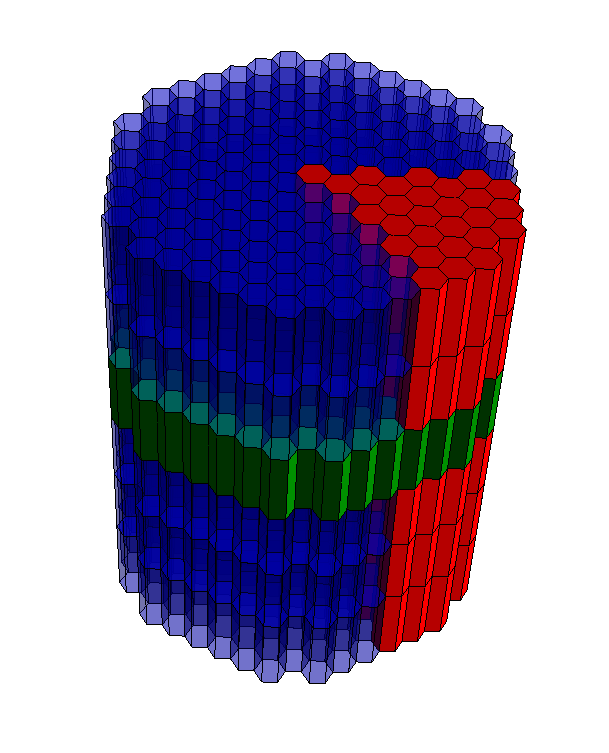
\includegraphics[scale=0.225]{obr/core.png}
  \column{.5\textwidth}
    \includegraphics<1>[scale=0.425]{obr/core/core_level1}
	  \includegraphics<2>[scale=0.425]{obr/core/core_level2}
	  \includegraphics<3>[scale=0.425]{obr/core/core_level3}
	  \includegraphics<4>[scale=0.425]{obr/core/core_level4}
	  \includegraphics<5>[scale=0.425]{obr/core/core_level5}
	  \includegraphics<6>[scale=0.425]{obr/core/core_level6}
	  \includegraphics<7>[scale=0.425]{obr/core/core_level7}
	  \includegraphics<8>[scale=0.425]{obr/core/core_level8}
	  \includegraphics<9>[scale=0.425]{obr/core/core_level9}
	  \includegraphics<10>[scale=0.425]{obr/core/core_level10}
	  \transduration<1-9>{0.5}
	  \transduration<10>{500}    
  \end{columns}
  \hfill\alert{3 dimenze}\hfill\hbox{}
\end{frame}

\begin{frame}[t]
  \frametitle{Stavový prostor}
  \framesubtitle{Energie}
 
  $$
    X = \VV \times \EE \times \SS \equiv \{x = (\br,\alert E,\bomega):\ \br\in \VV, \alert{E \in \EE}, \bomega\in \SS\}
  $$
  \vspace{.5em}
  \begin{columns}
  \column{.5\textwidth}
  \centering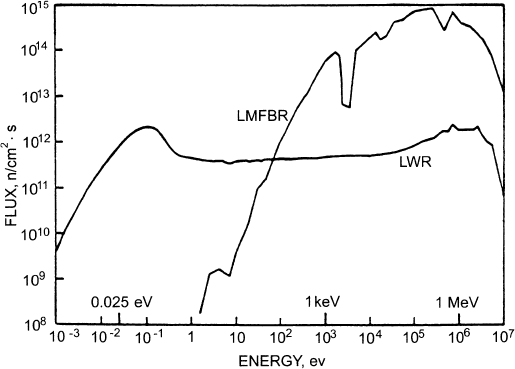
\includegraphics[width=.9\textwidth]{obr/spektrum}
  \column{.5\textwidth}
  \centering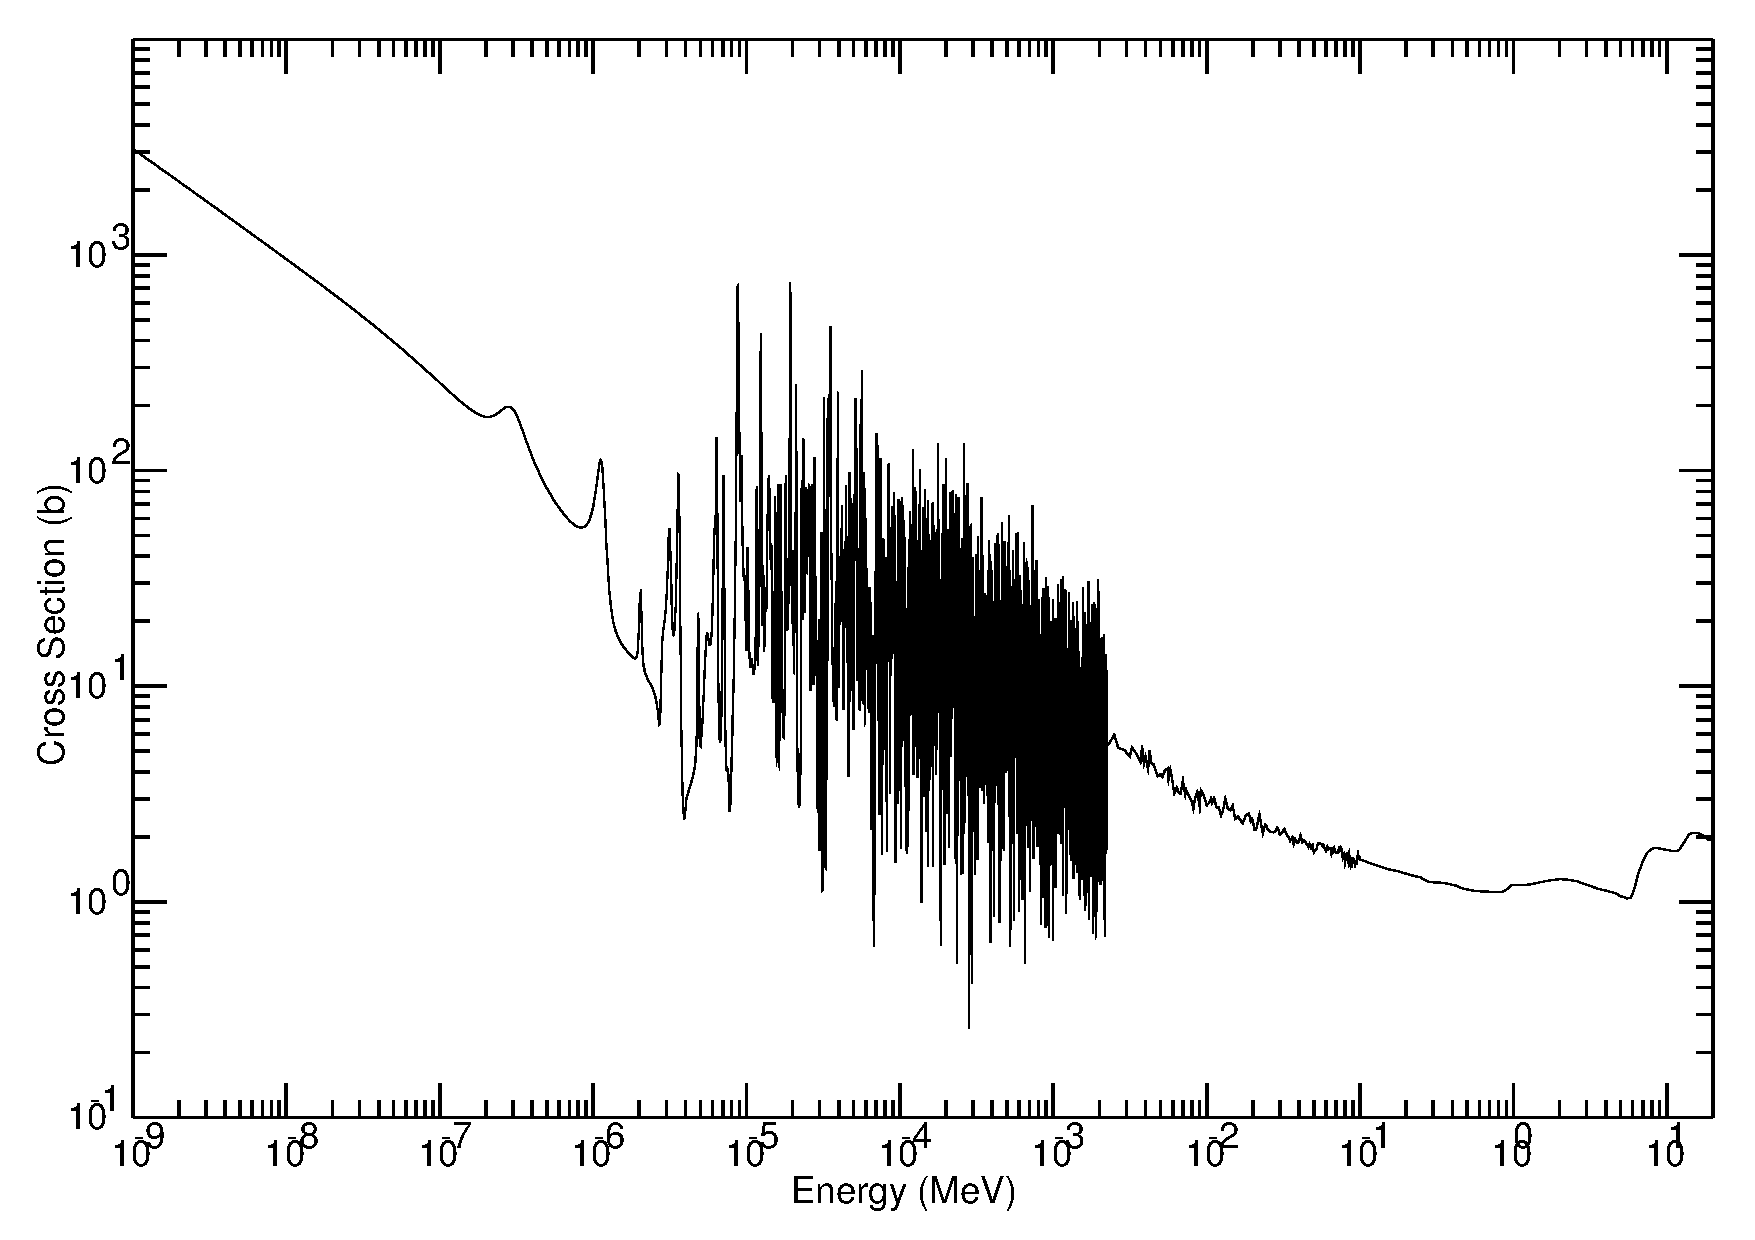
\includegraphics[width=.9\textwidth]{obr/U235f}
  \end{columns}
  \begin{center}
  \alert{1 dimenze}
  \end{center}
\end{frame}

\begin{frame}[t]
  \frametitle{Stavový prostor}
  \framesubtitle{Směr}
 
  $$
    X = \VV \times \EE \times \SS \equiv \{x = (\br,E,\alert\bomega):\ \br\in \VV, E \in \EE, \alert{\bomega\in \SS}\}
  $$
  
  
  \vspace{.5em}
  \begin{columns}
  \column{.5\textwidth}
  \centering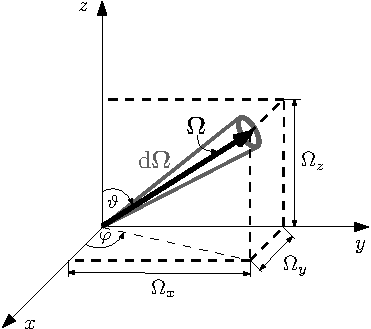
\includegraphics[width=.9\textwidth]{obr/cartesian_streaming}
  \column{.5\textwidth}
  \centering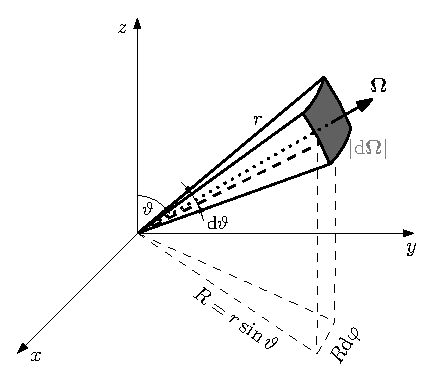
\includegraphics[width=.9\textwidth]{obr/element}
  \end{columns}
  \begin{center}
  \alert{2 dimenze}
  \end{center}
  
\end{frame}

\begin{frame}
  \frametitle{Základní směrově závislé veličiny}

  \begin{columns}[c]
  \begin{column}{.60\linewidth}  
    \begin{itemize}
    \item Hustota neutronů (v $\d{\br}\d{E}\d{\bomega}$):
    \begin{myitemize}
    	\item $N(\br,E,\bomega,t)$
    \end{myitemize}
  \end{itemize}
  \end{column}
  \begin{column}{.30\linewidth}  
  \end{column}
  \end{columns}
  
  \begin{columns}[c]
  \begin{column}{.60\linewidth}
  \begin{itemize}
	  \item Směrový neutronový tok
	  \begin{myitemize}
	    \item $\angflux(\br,E,\bomega,t) = v(E)N(\br,E,\bomega,t)$
	  	\item $\angflux(\br,E,\bomega,t)\,\d{\bomega}\d{E}$
	  \end{myitemize}
  \end{itemize}
  \end{column}
  \begin{column}{.30\linewidth}
  	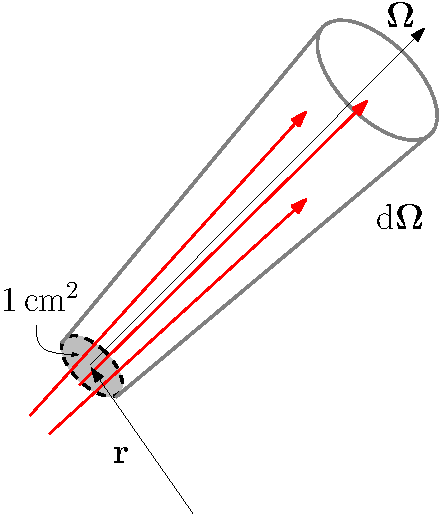
\includegraphics[scale=.45]{obr/angflux}
	\end{column}
	\end{columns}
	\vspace{-2em}
	\begin{columns}
	\begin{column}{.60\linewidth}
	\begin{itemize}
	  \item Směrový neutronový proud
	  \begin{myitemize}
	    \item $\bj(\br,E,\bomega,t) = \bomega \angflux(\br,E,\bomega,t)$\\
	  	\item $j(\br,E,\bomega,t) = \bn\cdot\bj(\br,E,\bomega,t)\,\d{S}\d{\bomega}\d{E}$
	  \end{myitemize}
  \end{itemize}
  \end{column}
  \begin{column}{.30\linewidth}
   	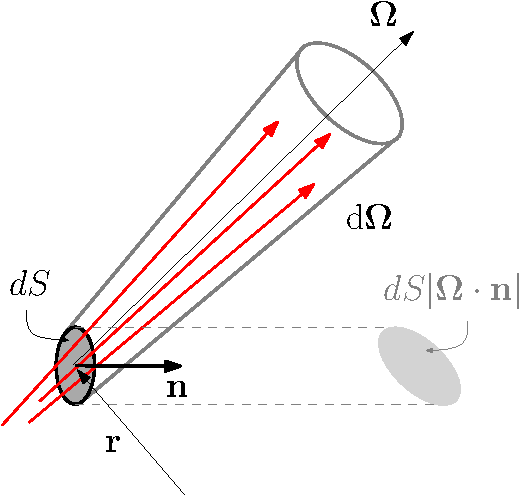
\includegraphics[scale=.45]{obr/angcur}
  \end{column}
  \end{columns}
\end{frame}

\begin{frame}
  \frametitle{Směrově nezávislé veličiny}
  \shorten{-.2em}{-.2em}
  \begin{itemize}
	  \item Skalární neutronový tok:
	    $$ \fl(\br,E,t) = \aint{\angflux(\br,E,\bomega,t)} $$
	  \item Úhrnný neutronový proud: 
	    $$\bJ(\br,E,t)	= \aint{\bj(\br,E,\bomega,t)} = \aint\bomega\angflux(\br,E,\bomega,t)$$
	  \item Parciální neutronový proud:
	    $$
	      j^{\pm}(\br,E,t) = \Aint[\bomega\cdot\bn \gtrless 0]{\abs{\bomega\cdot\bn}\angflux(\br,E,\bomega,t)}
	    $$
	    \vspace*{-.5em}
	  \begin{itemize}
	  	\item přestup neutronů
	  	  $\left.\begin{cases} \mbox{ve směru} &(j^+)\\
	  	    \mbox{proti směru} &(j^-)
	  	    \end{cases}\right\}$
	  	  vnější normály dané plochy
	  \end{itemize}
	  \vspace*{.5em}
	  \item Úhrnný neutronový proud (skalár): $j = \bJ\cdot\bn = j^+-j^-$
  \end{itemize}
\lengthen
\end{frame}

\begin{frame}
  \frametitle{Charakterizace interakcí}
    \begin{myitemize}
	  \item $\Sigma_t = \Sigma_a + \Sigma_f + \Sigma_s$
	  \begin{myitemize}
	  	\item funkce $\br$, $E$, $t$, ale ne $\bomega$ (izotropní prostředí -- stejné vlastnosti ve všech směrech)
	  \end{myitemize}
    \item Četnosti reakcí v objemu $\VV$ za časovou jednotku
	  \begin{myitemize}
	  	\item $\vint{\eint{\Sigma_{t,a,f,s}(\br,E,t)\fl(\br,E,t)}}$
	  \end{myitemize}
	  \item Změna energie a směru pohybu: $\chi(E'\ra E,\, \bomega'\ra\bomega)$
	  \begin{myitemize}
	  	\item štěpení -- \alert<2>{izotropní proces} v \alert<3>{izotropním prostředí}
	  	\begin{itemize}\vspace*{.25em}
	  		\item $\chi(E'\ra E, \alert<3>{\bomega'}\ra\alert<2>{\bomega}) = \alert<2>{\frac{1}{4\pi}}\chi_f(E'\ra E\alert<3>)$
	  	\end{itemize}
	  	\item rozptyl -- \alert<4>{anizotropní proces v izotropním prostředí}
	  	\begin{itemize}\vspace*{.25em}
	  		\item $\chi(E'\ra E, \alert<4>{\bomega'\ra\bomega}) = \chi_s(E'\ra E,\,\alert<4>{\bomega'\cdot\bomega})$
	  	\end{itemize}	  	
	  \end{myitemize}
  \end{myitemize}

\end{frame}



  \section{Bilance směrového neutronového toku}
    \begin{frame}[t]
  \frametitle{Bilance směrového neutronového toku}

  \alert<3>{Časová změna množství neutronů v elementu stavového prostoru $=$}
  \begin{itemize}
	  \item[$+$] \alert<4>{množství nově se objevivších neutronů}
	  \item[$-$] \alert<5>{množství zachycených neutronů}
	  \item[$-$] \alert<6>{množství neutronů uniklých přes hranici}
  \end{itemize}
  
  \uncover<2->{
    \vspace{1em}
    Pomocí $\angflux$, u nějž předpokládáme
    \begin{itemize}
    	\item spojitou diferencovatelnost vzhledem k $t$\uncover<7->{, $\br$}
    \end{itemize}
    \shorten{-.4em}{0em}
    \alt<1-9>{
    \begin{multline*}
      {\color<3>{red}\Vint{\Eint{\Aint{\frac{1}{v(E)}\pd{\angflux(\br,E,\bomega,t)}{t}}}}} = 
      {\color<4>{red}\Vint{\Eint{\Aint{P(\br,E,\bomega,t)}}}}\\
      - {\color<5>{red}\Vint{\Eint{\Aint{\Sigma_t(\br,E,\bomega,t)\angflux(\br,E,\bomega,t)}}}}\\
      - \alt<1-6>{
          {\color<6>{red}\int_{\bnd}\Eint{\Aint{\bj(\br,E,\bomega,t)\bn(\br)\d{S}}}}
        }{
          \alt<7>{
            \Vint{\Eint{\Aint{\nabla\cdot\bj(\br,E,\bomega,t)}}}
          }{
            \Vint{\Eint{\Aint{\bomega\cdot\nabla\angflux(\br,E,\bomega,t)}}}
          }
        }
     \end{multline*}
     }{
     \begin{align*}
      \frac{1}{v(E)}\pd{\angflux(\br,E,\bomega,t)}{t} &=
      P(\br,E,\bomega,t)\\[-.25em]
      &- \Sigma_t(\br,E,\bomega,t)\angflux(\br,E,\bomega,t)\\[.4em]
      &- \bomega\cdot\nabla\angflux(\br,E,\bomega,t)
      \end{align*}
     }
    \lengthen
    \uncover<8-10>{ \alt<8-9>{($\bomega$ nezávisí na $\br$ \only<9>{-- \alert{ale jen v kartézských souřadnicích!}})}{($\d{\br}\d{E}\d{\bomega}$ libovolné)} }
  }
\end{frame}

\begin{frame}
  \frametitle{Bilance směrového neutronového toku}
  \framesubtitle{Zdrojový člen}
    \shorten{-.35em}{-.35em}
    \begin{multline*}
    \frac{1}{v(E)} {\pd{\angflux(\br,E,\bomega,t)}{t}} = \\
    {\alert<2-3>{P(\br,E,\bomega,t)}}
    - {\Sigma_t(\br,E,\bomega,t)\angflux(\br,E,\bomega,t)}
    - {\bomega\cdot\nabla\angflux(\br,E,\bomega,t)}
    \end{multline*}
    \pause
    \temporal<3>{
      \begin{align*}
        {\alert{P(\br,E,\bomega,t)}} &= 
          \aintp{\eintp{\nu\Sigma_{\color{cyan}{f}}(\br,E',t)\chi_{\color{cyan}{f}}(E'\ra E,\, \bomega'\ra\bomega)\angflux(\br,E',\bomega',t)}}\\
          &+
          \aintp{\eintp{\Sigma_{\color{magenta}{s}}(\br,E',t)\chi_{\color{magenta}{s}}(E'\ra E,\, \bomega'\ra\bomega)\angflux(\br,E',\bomega',t)}}\\[.25em]
          &+
          {Q(\br,E,\bomega,t)}
      \end{align*}
    }{
      \begin{align*}   
        {\alert{P(\br,E,\bomega,t)}} &= 
          \frac{1}{4\pi}\eintp{\nu\Sigma_{\color{black}{f}}(\br,E',t)\chi_{\color{black}{f}}(E'\ra E){\color{black}\fl(\br,E',t)}}\\
          &+
          \aintp{\eintp{\Sigma_{\color{black}{s}}(\br,E',t)\chi_{\color{black}{s}}(E'\ra E,\, \bomega'\cdot\bomega)\angflux(\br,E',\bomega',t)}}\\[.25em]
          &+
          {Q(\br,E,\bomega,t)}
      \end{align*}
    }{
      \begin{align*}   
        {P(\br,E,\bomega,t)} &= 
          \frac{1}{4\pi}\eintp{{\color{red}
            \alt<4>{
              \nu\Sigma_f(\br,E',t)\chi_f(E'\ra E)
             }{
              \nu\Sigma_f(\br,E'\ra E,t)
             }}\fl(\br,E',t)}\\
          &+
          \aintp{\eintp{{\color{red}
            \alt<4>{
              \Sigma_s(\br,E',t)\chi_s(E'\ra E,\, \bomega'\cdot\bomega)
            }{
              \Sigma_s(\br,E'\ra E,\, \bomega'\cdot\bomega,t)
            }}\angflux(\br,E',\bomega',t)}}\\[.25em]
          &+
          {Q(\br,E,\bomega,t)}
      \end{align*}
    }   
    \lengthen
    \vspace*{-.4em}
    \uncover<3-5>{
      \begin{itemize}
      	\item předpoklady na izotropii
      	\item veškeré štěpení pro jednoduchost okamžité, bez zpožděných neutronů
      \end{itemize} 
    }     
\end{frame}


\begin{frame}
  \frametitle{Doplňující předpoklady a podmínky}
  \begin{itemize}
  	\item Pro skoro všechna $x\in X$: 
  	$$
  	\begin{gathered}
	    \begin{array}{ccl}
	    0 \leq& \!\!\!\Sigma_t(x,t)\!\!\! &< \infty,\\
	    0 \leq& \!\!\!\angflux(x,t)\!\!\! &< \infty,\\
	    0 \leq& \!\!\!Q(x,t)\!\!\! &< \infty,
	    \end{array}\\
	    \Sigma_t,\, \angflux\, \not\equiv 0.
	    \end{gathered}
    $$
    \item $\Sigma_t(\cdot,t)\in L^{\infty}(X)$,~ $\angflux(\cdot,t),\, Q(\cdot,t)\, \in \Lp{1}(X)$\vspace{.5em}
    \item $\aint{\eint{\chi_{s,f}(E'\ra E, \bomega'\ra \bomega)}} = 1$\vspace{.5em}
    \item Počáteční podmínka: $\angflux(\br,E,\bomega,t_0) = \Psi_0(\br,E,\bomega)$\vspace{.5em}
    \item Okrajové podmínky na \emph{\color{structure}vtokové hranici}
  \end{itemize}
  
  
\end{frame}

\begin{frame}
  \frametitle{Okrajové podmínky}
  \framesubtitle{Pomocné definice}
  
  \begin{itemize}
  	\item Homogenní / nehomogenní hranice: $\pV = \pVn \cap \pVh$
  	\hspace*{-3em}
  	\begin{minipage}{\paperwidth}
    $$
      \angflux_{\mathrm{in}}(\br,E,\bomega,t) = \begin{cases}
      \Psi_{\mathrm{in}}(\br,E,\bomega,t)\\
      0
      \end{cases}\hspace{-1em},\
      \angflux_h(\br,E,\bomega,t) = \begin{cases}
      0 & \br\in\pVn\\
      \Psi_h(\br,E,\bomega,t) & \br\in\pVh
      \end{cases}
    $$
    \end{minipage}\vspace{.75em}
    \item Vtoková / odtoková hranice:
  	$$
      \only<1>{\pX[\pm]}\only<2>{\pX[\pm]_{\;\color{red}0}}\only<3>{\pX[\pm]_{\,\color{red}h}} = 
        \bigl\{
          x = ({\color{cyan}\br}, {\color{magenta}E}, {\color{dkgreen}\bomega)}:
          {\color{cyan}\br \in \only<1>{\pV}\only<2>{\pV_{\color{red}0}}\only<3>{\pV_{\color{red}h}}},\ 
          {\color{magenta} E \in \EE},\ 
          {\color{dkgreen}\bomega\in\SS\land\bomega\cdot\bn(\br) \gtrless 0}
        \bigr\}
    $$
    \item Úhel zrcadlového odrazu (\emph{specular reflection}):
    \shorten{-.1em}{-1.5em}
    $$
      \bomega_R = \bomega - 2 \bn (\bomega \cdot \bn)
    $$
    \lengthen
    \begin{itemize}
    	\item Householderova transf. vektoru $\bomega$ vzhledem k rovině s normálou $\bn$
    	\item Úhel odrazu $=$ úhel dopadu:  $\abs{\bomega\cdot\bn} = \abs{\bomega_R\cdot\bn}$
    	\item Úhel odrazu leží ve stejné rovině jako úhel dopadu: $(\bomega_R\times\bn)\cdot\bn = 0$
    \end{itemize}
    
  \end{itemize}

\end{frame}

\begin{frame}
  \frametitle{Okrajové podmínky}
  \framesubtitle{Vybrané typy}
  $$
    \angflux(x,t) = \angflux_{\mathrm{in}}(x,t) + \alert<2->{\angflux_h(x,t)},\quad x = (\br,E,\bomega)\in\pX
  $$
  \pause
  \begin{itemize}
  	\item<3-> \alt<3>{Nonreentrantní}{Volná} hranice\uncover<5->{
  	-- rozhranní mezi zkoumaným prostředím a
    vakuem, příp. perfektním absorbérem (\emph{black body})
  	$$
  	  \angflux_h(x,t) = 0,\quad x\in\pX[-]_h
  	  \qquad (\Longrightarrow\ \ j^{-}(\br,E,t) = 0)
  	$$
  	}    
  	\item<6-> Zrcadlový odraz (\emph{specular reflection})
  	$$
  	  \angflux_h(x,t) = \angflux(\br,E,\bomega_R,t),\quad x\in\pX[-]_h
  	$$
  \end{itemize}

\end{frame}

\begin{frame}
  \frametitle{Okrajové podmínky}
  \framesubtitle{Vybrané typy}
  \shorten{-.5em}{-1em}
  $$
    \angflux(x,t) = \angflux_{\mathrm{in}}(x,t) + \alert<1-2>{\angflux_h(x,t)},\quad x = (\br,E,\bomega)\in\pX
  $$
  \lengthen
  \begin{itemize}
  	\item Okrajová podmínka typu albedo
  	$$
  	  \angflux_h(x,t) = \bndint[']{\pX[+]_h}\beta(x'\ra x,t)\angflux(x',t),\quad x\in\pX[-]_h,
  	$$
  	kde $\db{x'} = \abs{\bomega'\cdot\bn}\d{S}\d{E'}\d{\bomega'}$
  	
  	\uncover<2->{
  	\begin{myitemize}
  	 	\item $\beta$ charakterizuje případy, kdy v okamžiku $t$ neutron opouští prostředí\\
  	 	  v místě $\br'$, s energií $E'$ a ve směru $\bomega'$ a jiný neutron se vrací\\
  	 	  v jiném místě $\br$, s jinou energií $E$ a v jiném směru $\bomega$.
      \item Jiné typy podmínek lze získat lokalizací, např. zrcadlový odraz:\\[.3em]\centering 
        $\beta(\br'\ra \br, E'\ra E, \bomega'\ra\bomega,t) = \delta(\br' - \br)\delta(\bomega' - \bomega_R)\delta(E' - E)$
  	 \end{myitemize}\vspace{.2em}
  	}
  	\item<3-> Spojitost směrového toku na vnitřních rozhranních ($\forall E,\ \bomega$)
  \end{itemize}

\end{frame}

%TODO: White B.C, isotropic reflection, source condition


  \section{Různé podoby rovnice transportu neutronů}
    \begin{frame}
  \frametitle{Ustálený stav}
  
    \begin{multline*}
    \frac{1}{v(E)} {\pd{\angflux(\br,E,\bomega,t)}{t}} = \\
    {P(\br,E,\bomega,t)}
    - {\Sigma_t(\br,E,\bomega,t)\angflux(\br,E,\bomega,t)}
    - {\bomega\cdot\nabla\angflux(\br,E,\bomega,t)}
    \end{multline*}
    + počáteční a okrajové podmínky
    \uncover<2>{
    \begin{center}
    \begin{tikzpicture}
      \draw[decorate, decoration=snake,thick,structure,->] (0,0) -- (0,-1);
    \end{tikzpicture}
    \end{center}
    $$
      \bomega\cdot\nabla\angflux(\br,E,\bomega) +
      \Sigma_t(\br,E,\bomega)\angflux(\br,E,\bomega) =
      P(\br,E,\bomega)
    $$
    \\[.5em]
    + okrajové podmínky
    }

\end{frame}

\begin{frame}
  \frametitle{Operátorový zápis}
  \framesubtitle{integro-diferenciální LBR}
  
$$
  \left\{
    \begin{aligned}
       \alert<2-3>{L\angflux} &= P \equiv \alert<4>{H\angflux} + \alert<5>{F\angflux} + \alert<6>{Q}\quad &&\mbox{ v $X$,}\\
	  \angflux  &= \alert<7>{\beta\angflux} + \angfluxin\quad   &&\mbox{ na $\pX[-]$.}
    \end{aligned}
  \right.
$$
\begin{itemize}
	\item<2-> \alert<2>{advekce} a \alert<3>{záchyt}: $(\alert<2-3>{L\angflux})(x) = \alert<2>{\bomega\cdot\nabla\angflux(x)} + \alert<3>{\Sigma_t\angflux(x)}$
	\item<4-> \alert<4>{rozptyl} a \alert<5>{stěpení}: 
	    \begin{align*}
		      (\alert<4>{H\angflux})(x) &= \aintp{\eintp{\Sigma_s(\br, E'\ra E, \bomega'\cdot\bomega)\angflux(\br,E',\bomega')}}\\
		      (\alert<5>{F\angflux})(x) &= \frac{1}{4\pi}\eintp{\nu\Sigma_f(\br, E'\ra E)\aintp{\angflux(\br,E',\bomega')}}
      \end{align*}
	\item<6-> \alert<6>{stálý vnější neutronový zdroj:} $\alert<6>{Q(x)}$
	\item<7-> \alert<7>{přestup přes okraje:}
	$$
		(\alert<7>{\beta\angflux})(x) = \bndint[']{\pX[+]}\beta(\br'\ra \br, E'\ra E, \bomega'\ra\bomega)\angflux(\br', E', \bomega')
  $$
\end{itemize}

\end{frame}

\begin{frame}
  \frametitle{Úloha na $\keff$}
  
  $$
  \left\{
    \begin{aligned}
       (L-H)\angflux &= \frac{1}{\keff} F\angflux &&\mbox{ v $X$,}\\
	  \angflux  &= \beta\angflux \quad   &&\mbox{ na $\pX[-]$.}
    \end{aligned}
  \right.
$$

\end{frame}

\begin{frame}
  \frametitle{Mnohagrupová integro-diferenciální LBR}
  
  \vspace{-1.25em}
  
  \hbox{}\hfill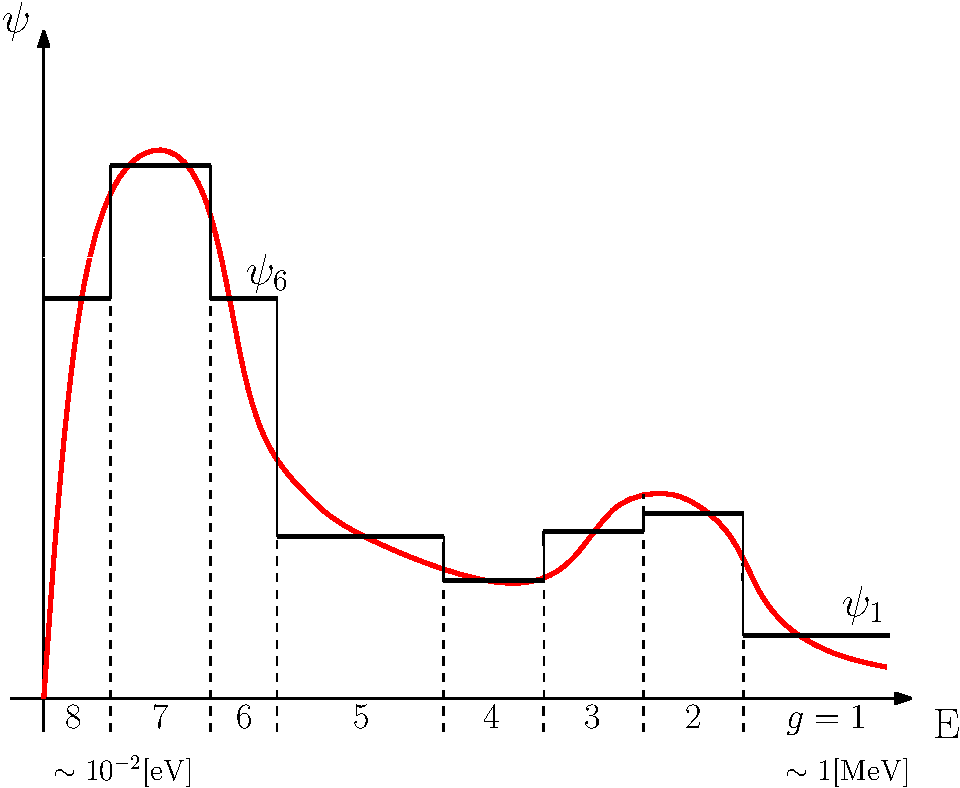
\includegraphics[width=.425\textwidth]{obr/fluxg}\hfill
  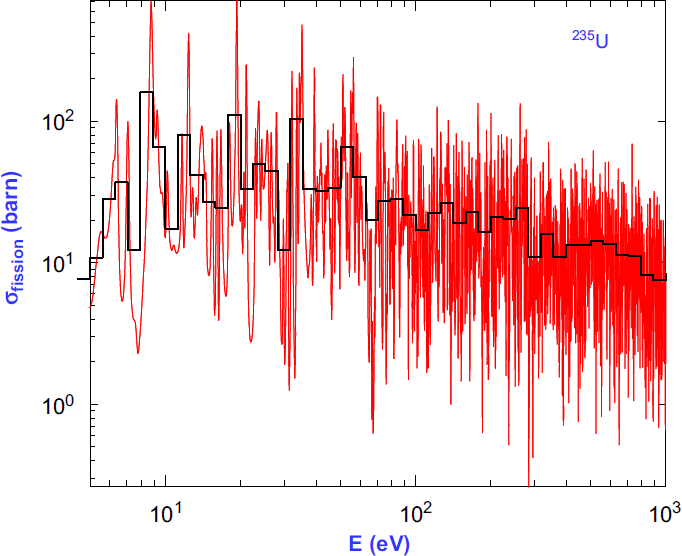
\includegraphics[width=.425\textwidth]{obr/U235fg}\hfill\hbox{}
  
  \shorten{-.6em}{0em}

  $$
  \left\{
    \begin{aligned}
    \llop\vangflux &= \hhop\vangflux + \ffop\vangflux + \QQ\quad &&\mbox{ v $X$,}\\
    \vangflux  &= \valbedo\vangflux + \vangflux_{\mathrm{in}}\quad   &&\mbox{ na $\pX[-]$}.
  \end{aligned}
  \right.
  $$

  \begin{gather*}
    \vangflux = \big[\angflux_g\big]_{g=1,\ldots, G}\quad
    \vangflux_{\mathrm{in}} = \big[\angflux_{\mathrm{in},g}\big]_{g=1,\ldots, G}\quad
    \QQ = \big[Q_g\big]_{g=1,\ldots, G}\\[.3em] 
    \llop = \big\llbracket L_{gg} \big\rrbracket_{g=1,\ldots, G} \\[.2em]
    \hhop = \big\llbracket H_{gg'}\big\rrbracket_{g,g'=1,\ldots, G} \quad
    \ffop = \big\llbracket F_{gg'}\big\rrbracket_{g,g'=1,\ldots, G} \quad
    \valbedo = \big\llbracket \beta_{gg'}\big\rrbracket_{g,g'=1,\ldots, G}
  \end{gather*}
  
  \lengthen
    
\end{frame}

\begin{frame}
  \frametitle{Monoenergetická podoba}
  
\begin{itemize}
	\item $ G = 1$,~ $\angflux = \angflux(\br,\bomega)$
	\item advekce a záchyt: $(L\angflux)(\br,\bomega) = \bomega\cdot\nabla\angflux(\br,\bomega) + \Sigma_t(\br)\angflux(\br,\bomega)$
	\item rozptyl a stěpení: 
	    \begin{align*}
		      (H\angflux)(\br,\bomega) &= \aintp{\Sigma_s(\br, \bomega'\cdot\bomega)\angflux(\br,\bomega')}\\
		      (F\angflux)(\br,\bomega) &= \frac{1}{4\pi}\nu\Sigma_f(\br)\aintp{\angflux(\br,\bomega')} = \frac{1}{4\pi}\nu\Sigma_f(\br)\fl(\br)
      \end{align*}
	\item stálý vnější neutronový zdroj: $Q(\br,\bomega)$
	\item přestup přes okraje: 
	$$
		(\beta\angflux)(x) = \bndint[']{\pX[+]}\beta(\br'\ra \br,\bomega'\ra\bomega)\angflux(\br',\bomega').
  $$
\end{itemize}

\end{frame}

\begin{frame}
  \frametitle{Integrální tvar}
  
\begin{itemize}
  \item Nechť $s\in I$ parametrizuje dráhu letu paralelního svazku neutronů
  \item V kartézské soustavě: $\der{x}{s} = \bomega_x,\ \der{y}{s} = \bomega_y,\ \der{z}{s} = \bomega_z$
	\item<2-> Označme $\Gamma = \{\br\in\RR[3]: \br = \br(s),\ s\in I\}$ ~(\emph{\color{structure}charakteristika})
	\item<3-> Platí
	  \begin{columns}
	  \column{.75\textwidth}
	    \begin{align*}
	      \bomega\cdot\nabla\angflux &= \bomega_x\pd{\angflux}{x} + 
	      \bomega_y\pd{\angflux}{y} + \bomega_z\pd{\angflux}{z}\\
	      & = 
	      \der{x}{s}\pd{\angflux}{x} + \der{y}{s}\pd{\angflux}{y} + \der{z}{s}\pd{\angflux}{z}
	      = 
	      \der{\angflux}{s}
	    \end{align*}
	  \column{.25\textwidth}
	  \hspace{-1.25em}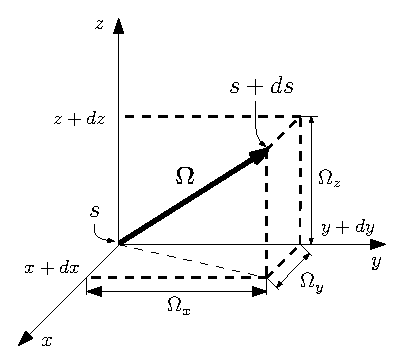
\includegraphics[width=1.15\textwidth]{obr/cartesian_streaming2}
	  \end{columns}\vspace{1em}
  \item<4-> $L\angflux \equiv \bomega\cdot\nabla\angflux + \Sigma_t\angflux = P\quad \Longrightarrow\quad \angflux = \alert<5>{L^{-1}}P$ \uncover<5->{\\(\alert<5>{umíme na charakteristikách})}
\end{itemize}

\end{frame}

\begin{frame}
  \frametitle{Integrální tvar}
  
  \begin{myitemize}
    \item Rovnice na charakteristice:~ $\der{\angflux(\br,\bomega)}{s} + \Sigma_t(\br,\bomega)\angflux(\br,\bomega) = P(\br,\bomega)$
    \item Řešení:~~ $\angflux(\br,\bomega) = \angflux(\br_0,\bomega)e^{-\tau(\br,\br_0)} + \int_0^{s_0} P(\br',\bomega)e^{-\tau(\br,\br')}\,\d{s'}$
    \begin{itemize}
    	\item $\br' = \br - s' \bomega$,~ $\br_0 = \br - s_0 \bomega$\\[.2em]
    	\item $\tau(\br,\br') = \tau(\br,\br-s'\bomega) = \int_0^{s'} \Sigma_t(\br - s''\bomega)\,\d{s''}$
    \end{itemize}
  \end{myitemize}
  \vspace{-.5em}
  \begin{center}
    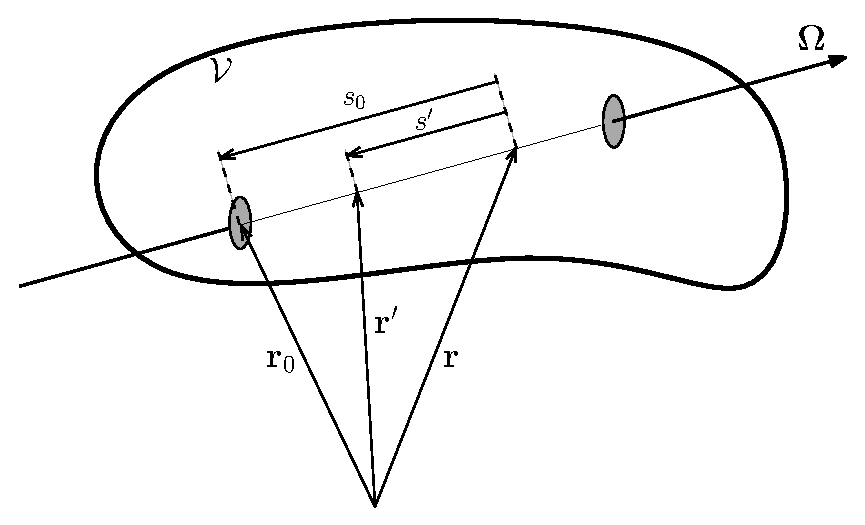
\includegraphics[scale=.5]{obr/trepka}
  \end{center}
  \vspace{-1em}
\end{frame}

\begin{frame}
  \frametitle{Integrální tvar}
  $$
    \angflux(\br,\bomega) = {\color<1>{red}\angflux(\br_0,\bomega)e^{-\tau(\br,\br_0)}} + {\color<2>{red}\int_0^{s_0} P(\br',\bomega)e^{-\tau(\br,\br')}\,\d{s'}}
  $$\\[1em]
  \ldots\ \alert<1>{neutrony, jež vstoupily do $\VV$ v $\br_0$ a dolétly do $\br$ (nebyly zachyceny)}\\
  $\hphantom{\ldots\ }$ + \alert<2>{neutrony ze zdrojů mezi $\br_0$ a $\br$, které nebyly zachyceny a dolétly do $\br$}\\
  $\hphantom{\ldots\ }$ (všechny uvažované neutrony letěly ve směru $\bomega$)
  \vspace{1em}
  \begin{itemize}[<3>]
    \item Na této formulaci jsou založeny např.
    \begin{itemize}
    	\item metoda charakteristik (MOC)
    	\item metoda kolizních pravděpodobností (CP)
    	\item nepřímo i metoda Monte Carlo (MC)
    \end{itemize}
  \end{itemize}


\end{frame}

\begin{frame}
  \frametitle{Trasování pohybu neutronů v integrálních metodách}
  \framesubtitle{Monte Carlo}
  \begin{center}
    \includegraphics<1>[scale=.5]{obr/MC}
    \includegraphics<2>[scale=.5]{obr/MC2}
  \end{center}
\end{frame}

\begin{frame}
  \frametitle{Trasování pohybu neutronů v integrálních metodách}
  \framesubtitle{Metoda (dlouhých) charakteristik}
  \vspace{-.4em}
  \begin{center}
    \includegraphics<1>[scale=.5]{obr/MOC}
    \includegraphics<2->[scale=.25]{obr/MOC2}
  \end{center}
  \only<2->{\vspace{-1.4em}}
  \begin{itemize}
    \only<1>{\item Geometrické informace (délky segmentů) lze spočíst nezávisle na $\angflux$}
  	\only<2->{\item Výpočet $\angflux_i(\bomega) = \Vint[\VV_i]{\angflux(\br,\bomega)}$ pro každou zónu nasčítáním příspěvků z jednotlivých charakteristik ve směru $\bomega$ (kvadratura pro prostor. int.)}
  	\item<3> Výpočet $\flux_i = \Vint{\flux(\br)}$ pro každou zónu nasčítáním $\angflux_i(\bomega)$ z charakteristik v jednotlivých směrech (kvadratura pro int. přes směry)
  \end{itemize}
  
\end{frame}



  \section{Rovnice "doleva/doprava"}
    \begin{frame}
  \frametitle{Transport neutronů ve dvou směrech}
  
  \begin{myitemize}
    \item Monoenergetický, ustálený stav, pro jednoduchost bez štěpení
    \begin{itemize}
    	\item $\Sigma_t = \Sigma_a + \Sigma_s$
    \end{itemize}
	  \item Pohyb neutronů omezen do dvou směrů:
	  $$
	    \bomega \equiv \bomega_x \equiv \mu = 
	    \begin{cases}
	      +1 & \quad \mbox{(kladná poloosa $x$)},\\
	      -1 & \quad \mbox{(záporná poloosa $x$)}
	    \end{cases}
	  $$
	  \item<2-> $\angflux_{\pm}(x) = \angflux(x,\pm 1)$
	  \item<2-> $\flux(x) = \angflux_+(x) + \angflux_-(x)$
	  \item<2-> $J(x) = (+1)\angflux_+(x) + (-1)\angflux_-(x) = \angflux_+(x) - \angflux_-(x)$
	  \item<2-> $Q_\pm = Q(x,\pm 1)$
  \end{myitemize}

\end{frame}

\begin{frame}
  \frametitle{Transport neutronů ve dvou směrech}
  \framesubtitle{Rozptyl}
    \vspace{-1em}
	  \begin{gather*}
      \Sigma_s(x,\mu'\ra\mu) = 
      \begin{cases}
        \Sgmr(x) & \ \; \mu'\mu = +1,\\
        \Sgml(x) & \ \; \mu'\mu = -1,
      \end{cases}\\[.5em]
	    \Sigma_s(x) = \Sgml(x) + \Sgmr(x)
    \end{gather*}

    \begin{itemize}
    	\item střední hodnota kosinu rozptylového úhlu:
    	$$
    	  \muav = \frac{(+1)\Sgmr + (-1)\Sgml}{\Sgmr + \Sgml} = \frac{\Sgmr - \Sgml}{\Sigma_s}
    	$$
    	\item<2-> izotropní rozptyl: $$\Sgmr = \Sgml = \frac{\Sigma_s}{2}\quad \Longrightarrow\quad \muav = 0$$
    	\item<2-> bez rozptylu (neutrony nemění při kolizích směr):
          	$$\Sigma_s = \Sgmr \quad \Longrightarrow\quad \muav = 1$$
    \end{itemize}

\end{frame}

\begin{frame}
  \frametitle{Lineární Boltzmannova rovnice v dvousměrovém modelu}

    $$
      \pm\der{\angflux_{\pm}(x)}{x} + \Sigma_t(x)\angflux_{\pm}(x) = 
      \Sgmr(x)\angflux_{\pm}(x) + \Sgmr(l)\angflux_{\mp}(x) + Q_{\pm}(x)
    $$
    

    \begin{itemize}
    	\item<2-> sečtením obou rovnic ~~~ (označ. $Q = Q_+ + Q_-$):
    	$$
    	  \der{J}{x} + \Sigma_t\flux = \Sigma_s\flux + Q
    	  \quad\Longrightarrow\quad
    	  \der{J}{x} + \Sigma_a\flux = Q
    	$$
    	\item<3-> odečtením obou rovnic ~ (označ. $J_Q = Q_+ - Q_-$):
    	$$
    	  \der{\flux}{x} + \Sigma_t J = \muav\Sigma_s J + J_Q
    	  \quad\Longrightarrow\quad
    	  J = -\frac{1}{\Sigma_t-\muav\Sigma_s}\left(\der{\flux}{x} - J_Q\right)
    	$$
    	\item<4->[$\Rightarrow$] S využitím standardních definic \alert<5>{klasické difúzní teorie}:
    	$$
    	  D = \frac{1}{\only<5>{\alert3}\Sigma_{tr}} = \frac{1}{\only<5>{\alert{3(}}\Sigma_t-\muav\Sigma_s\only<5>{\alert)}}
    	$$
    	nakonec dostaneme LBR ve tvaru
    	$$
    	  -\der{}{x}\bigg[D(x)\der{\flux(x)}{x}\bigg] + \Sigma_a(x)\flux(x) = Q(x) - \der{}{x}\bigg[D(x)J_Q(x)\bigg]
    	$$
    	\end{itemize}

\end{frame}

\begin{frame}
  \frametitle{Lineární Boltzmannova rovnice v dvousměrovém modelu}
  \framesubtitle{Doplňující podmínky a vztahy}
    \vspace{.75em}\centering $\VV = (x_{b-}\;,\; x_i)\; \cup\; (x_i\; ,\; x_{b+})$\\[.25em]
    \begin{itemize}
    	\item Okrajová podmínka na volné hranici:
        $$
        \angflux_\mp(x_{b\pm}) = 0\quad \Longrightarrow\quad \mp D\left.\der{\flux}{x}\right\vert_{x_{b\pm}} = \left.\vphantom{\der{\flux}{x}}\big(\flux \mp D J_Q\big)\right\vert_{x_{b\pm}}
    		$$
    	\item Podmínky na vnitřních rozhraních:
    	\begin{myitemize}
    		\item $0 = \Delta(\angflux) := \lim\limits_{x\to x_i+}\angflux_\pm(x) - \lim\limits_{x\to x_i-}\angflux_\pm(x)$
    		\item $\Delta\bigg(D\der{\flux}{x}\bigg) = \Delta(D J_Q)$
    	\end{myitemize}\vspace{.5em}
    	\item Vztah mezi směrovými toky skalárním tokem:
    	$$
  	    \angflux_\pm(x) = \frac12\bigg[\flux(x) \pm J(x)\bigg] = \frac12\bigg[\flux(x)\mp D(x)\der{\flux(x)}{x} \pm D(x)J_Q(x)\bigg]
    	$$  	
    \end{itemize}

\end{frame}

\begin{frame}
  \frametitle{Lineární Boltzmannova rovnice v dvousměrovém modelu}
  \framesubtitle{Difúzní podoba}
      
      \textcolor{structure}{\emph{Pro izotropní zdroje}} ($J_Q = 0$) máme formálně \alert<2>{klasickou rovnici difúze neutronů} v samoadjungovaném tvaru
    	$$
    	  -\der{}{x}\bigg[D(x)\der{\flux(x)}{x}\bigg] + \Sigma_a(x)\flux(x) = Q(x)
    	$$
    	s extrapolovanou okrajovou podmínkou na volné hranici:
    	$$
      	\mp \left.\frac{1}{\flux}\der{\flux}{x}\right\vert_{x_{b\pm}} = \frac{1}{\only<2->{\alert{2}}D(x_{b\pm})} = \only<2->{\alert{\frac32}}\Sigma_{tr}(x_{b\pm})
    	$$
    	a spojitostí proudů a toků na vnitřních rozhraních
    	
\end{frame}

\begin{frame}
  \frametitle{Příklad 1 -- v prostoru rozložený izotropní zdroj}
  \framesubtitle{Data}
  
  \centering$a = 5$\,cm\\[1em]
  \centering$\VV = \textcolor{matCdk}{(-\infty, -a)} \; \cup \; \textcolor{matBdk}{(-a,a)} \; \cup \; \textcolor{matCdk}{(a,+\infty)}$

\begin{center}
	\begin{tabular}{|ABC|}
	  \hline
		 & $\abs{x} < a$ & $\abs{x} > a$ \nl
		$\Sigma_t\,[\mathrm{cm}^{-1}]$ & 1.00 & 0.50 \nl
		$\Sigma_a\,[\mathrm{cm}^{-1}]$ & 0.55 & 0.10 \nl
		$Q\,[\mathrm{cm}^{-1}s^{-1}]$ & 0.10 & 0.00 \nl
		$\muav$ & $\textcolor<2>{blue}{\bar\mu_{01}}$ & $\textcolor<2>{blue}{\bar\mu_{02}}$
		\nl
	\end{tabular}
\end{center}

\end{frame}

\begin{frame}
  \frametitle{Příklad 1 -- v prostoru rozložený izotropní zdroj}
  \framesubtitle{$\bar\mu_{01} = 0.75$~~~~$\bar\mu_{02} = 0.5$}
  
	\centering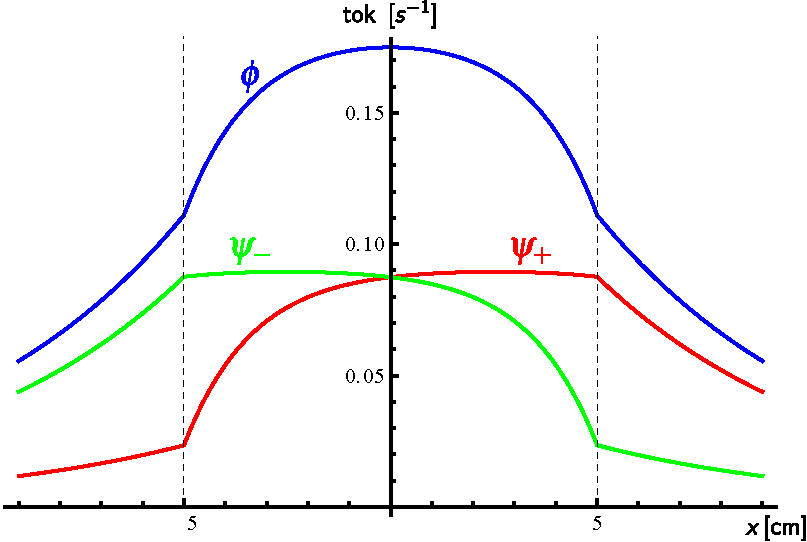
\includegraphics[height=.8\paperheight]{obr/doleva_doprava/distribuovany_075_05}

\end{frame}

\begin{frame}
  \frametitle{Příklad 1 -- v prostoru rozložený izotropní zdroj}
  \framesubtitle{$\bar\mu_{01} = 0$ (izotropní rozptyl)~~~~$\bar\mu_{02} = 0.5$}
  
  \centering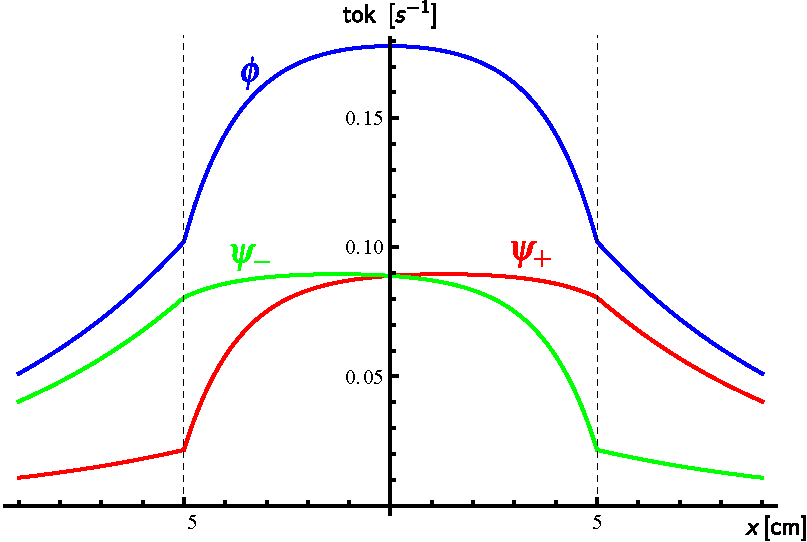
\includegraphics[height=.8\paperheight]{obr/doleva_doprava/distribuovany_0_05}

\end{frame}

\begin{frame}
  \frametitle{Příklad 1 -- v prostoru rozložený izotropní zdroj}
  \framesubtitle{$\bar\mu_{01} = 1$ (bez rozptylu)~~~~$\bar\mu_{02} = 0.5$}
  
  \centering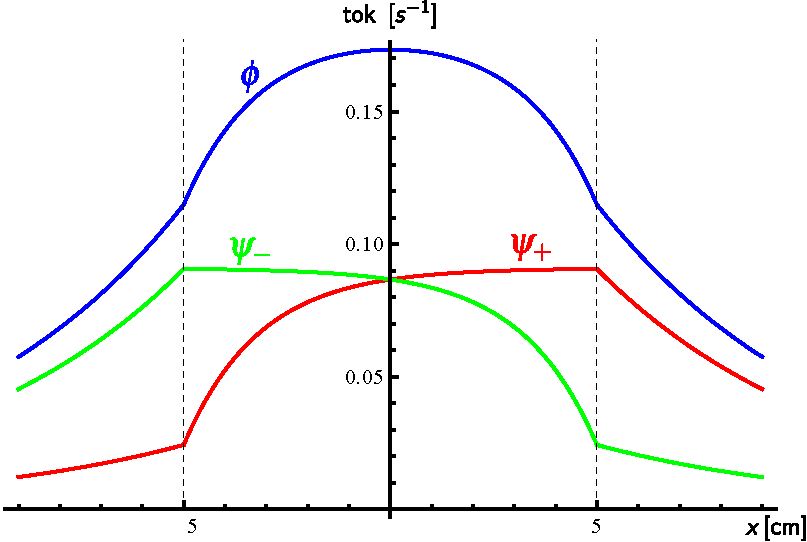
\includegraphics[height=.8\paperheight]{obr/doleva_doprava/distribuovany_1_05}

\end{frame}

\begin{frame}
  \frametitle{Příklad 1 -- v prostoru rozložený izotropní zdroj}
  \framesubtitle{$\bar\mu_{01} = 0.75$~~~~$\bar\mu_{02} = 1$ (bez rozptylu)}
  
  \centering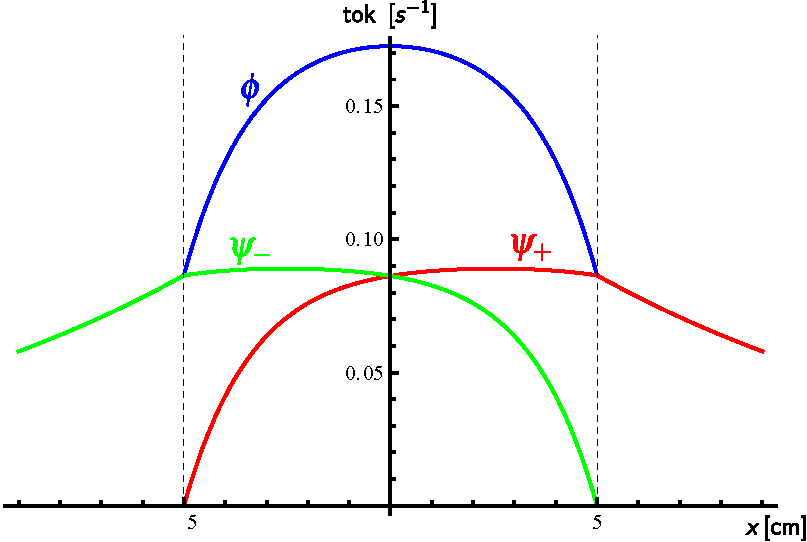
\includegraphics[height=.8\paperheight]{obr/doleva_doprava/distribuovany_075_1}

\end{frame}

\begin{frame}
  \frametitle{Příklad 1 -- v prostoru rozložený izotropní zdroj}
  \framesubtitle{$\bar\mu_{01} = 1$ (bez rozptylu)~~~~$\bar\mu_{02} = 1$ (bez rozptylu)}
  
  \centering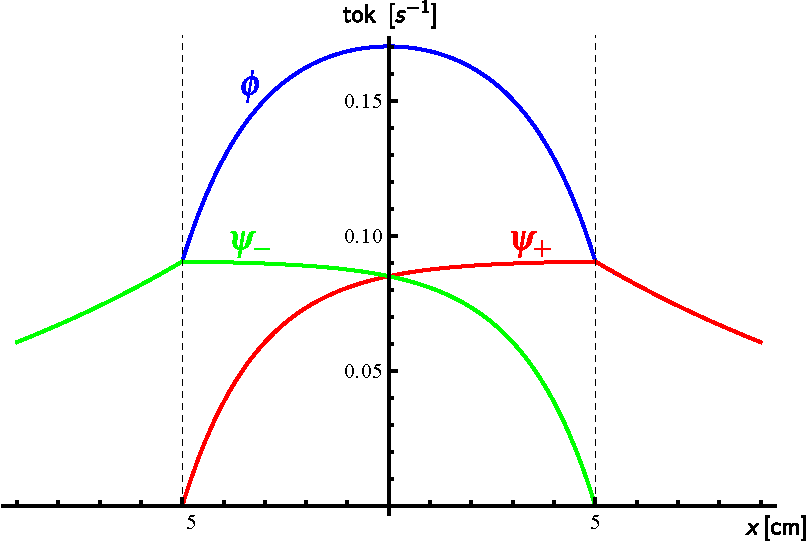
\includegraphics[height=.8\paperheight]{obr/doleva_doprava/distribuovany_1_1}

\end{frame}

\begin{frame}
  \frametitle{Příklad 2 -- bodový anizotropní zdroj}
  \framesubtitle{Data}
  
  \centering $\VV = (0,a)$~ ve vakuu\\
  
  \begin{myitemize}
  	\item $a = 5$\,cm
  	\item $\Sigma_t = 1$\,cm$^{-1}$,~ $\Sigma_a = 0.5$\,cm$^{-1}$
  	\item $S_+ = 0.7$\,s$^{-1}$,~ $S_- = 0.3$\,s$^{-1}$\\[.5em]
  	      $Q_\pm(x) = S_\pm\delta(x-x_Q)$ [cm$^{-1}$s$^{-1}$]\\[.5em]
  	      $x_Q=2$\,cm
  	\item $\muav = \textcolor<2>{blue}{\bar\mu_{01}}$
  \end{myitemize}


\end{frame}

\begin{frame}
  \frametitle{Příklad 2 -- bodový anizotropní zdroj}
  \framesubtitle{$\bar\mu_{01} = 0.75$}
  
  \centering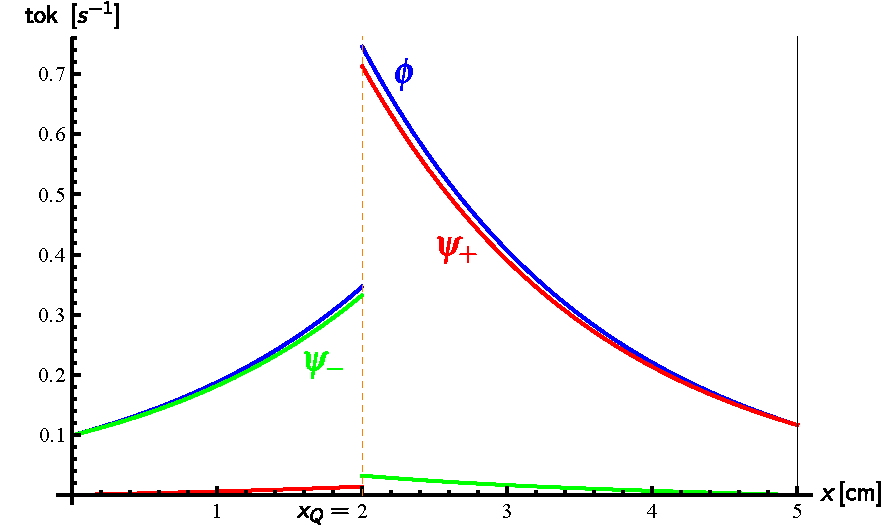
\includegraphics[height=.75\paperheight]{obr/doleva_doprava/bodovy_075}

\end{frame}

\begin{frame}
  \frametitle{Příklad 2 -- bodový anizotropní zdroj}
  \framesubtitle{$\bar\mu_{01} = 0$ (izotropní rozptyl)}
  
  \centering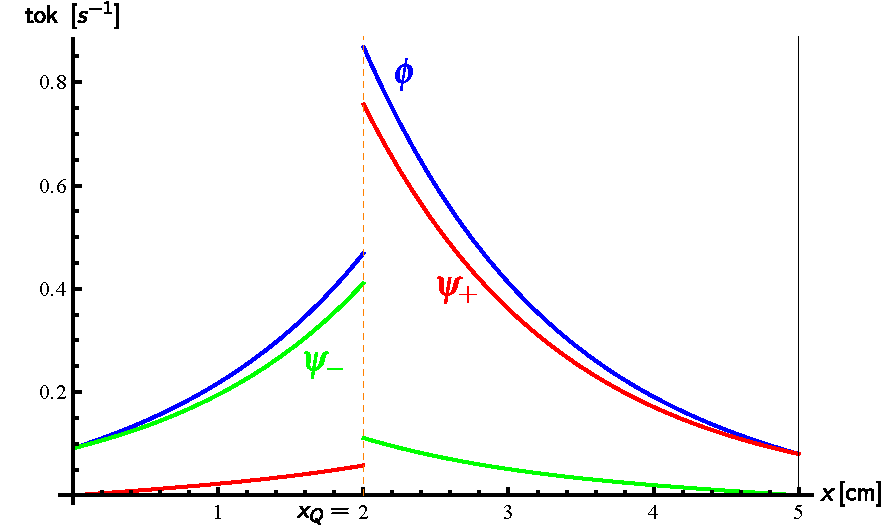
\includegraphics[height=.75\paperheight]{obr/doleva_doprava/bodovy_0}

\end{frame}

\begin{frame}
  \frametitle{Příklad 2 -- bodový anizotropní zdroj}
  \framesubtitle{$\bar\mu_{01} = 1$ (bez rozptylu)}
  
  \centering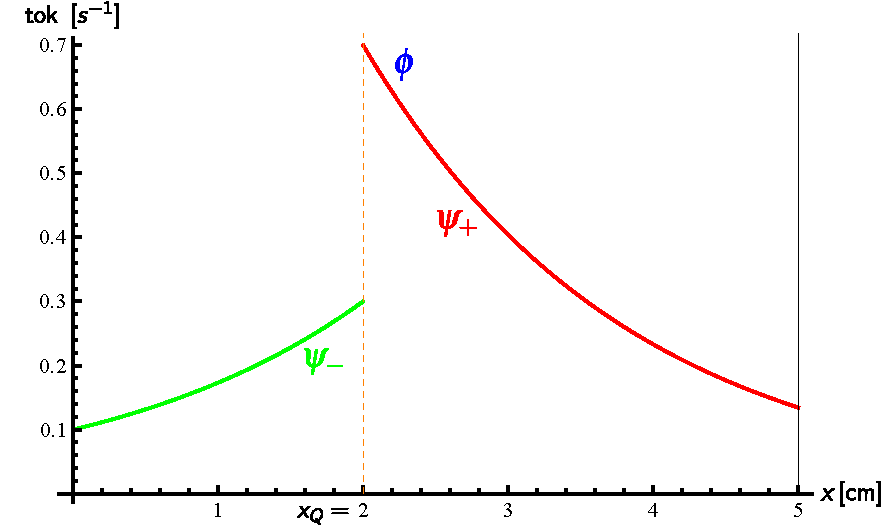
\includegraphics[height=.75\paperheight]{obr/doleva_doprava/bodovy_1}

\end{frame}

%\begin{frame}
%  \frametitle{Příklad -- v prostoru rozložený anizotropní zdroj}
%  \framesubtitle{Popis a tvar řešení}
%
%
%\end{frame}
%
%\begin{frame}
%  \frametitle{Příklad -- v prostoru rozložený anizotropní zdroj}
%  \framesubtitle{Průběh neutronových toků}
%
%
%\end{frame}

  \section{Matematická reprezentace směrové závislosti}
    \begin{frame}[t]
  \frametitle{Geometrie rozptylu}
  \vspace{.2em}
  \begin{itemize}
  	\item Anizotropní rozptyl v \textcolor{structure}{\emph{izotropním prostředí}} je vyjádřen funkcí \alt<1>{$\chi_s$}{\alert<2>{$\Sigma_s$}}:
  	\begin{overlayarea}{\textwidth}{2.35em}
  	\shorten{-.5em}{-.5em}
  	$$
  	  \alt<1>{
  	    \chi_s(\bomega'\ra\bomega) = \chi_s(\bomega\ra\bomega') = \chi_s(\bomega'\cdot\bomega) = \chi_s(\mu_0)
  	  }{
  	    \alert<2>{\Sigma_s(\br,\bomega'\ra\bomega)} = \Sigma_s(\br,\bomega\ra\bomega') = \Sigma_s(\bomega'\cdot\bomega) = \Sigma_s(\mu_0)
  	  },
  	$$
  	\lengthen
  	\end{overlayarea}
  	kde $\mu_0 = \cos \vartheta_0$ ~(kosinus rozptylového úhlu)\\[.5em]
  	
  	\only<1>{
      \centering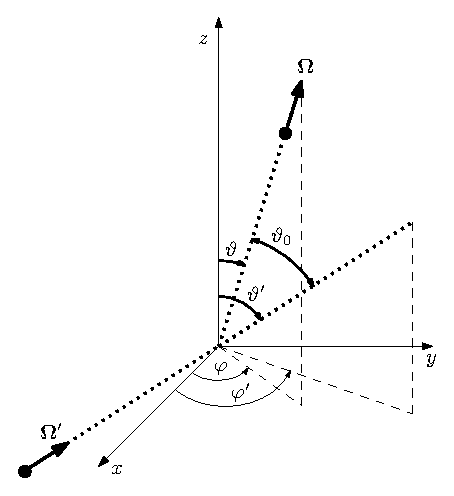
\includegraphics[scale=.75]{obr/scattering}
    }
  	\item<3->[$\Rabullet$] k popisu rozptylu nepotřebujeme zkoumat kartézský součin dvou sfér, nýbrž jen interval $[-1,1]$\\[1em]
  	\item<4-> V Hilbertově prostoru $\mathcal{H}([-1,1])$ můžeme funkci $\Sigma_s(\mu_0)$ ekvivalentně zapsat ve tvaru (zobecněného) Fourierova rozvoje vzhledem ke vhodné \alert<6>{úplné ortogonální bázi}
  	\item<5-> S jeho pomocí se budeme snažit vyjádřit \emph{\textcolor{structure}{rotačně invariantní}} operátor rozptylu $H$:
  	$$
  	  (H\angflux)(\br,\bomega) = \aintp{
        \Sigma_s(\br, \bomega'\cdot\bomega)
        \angflux(\br,\bomega')
      }
  	$$
  	ve finitní podobě (implementovatelné do počítače)
  \end{itemize}

\end{frame}

\begin{frame}
  \frametitle{Legendreovy polynomy}
  \vspace{-1em}
  \centering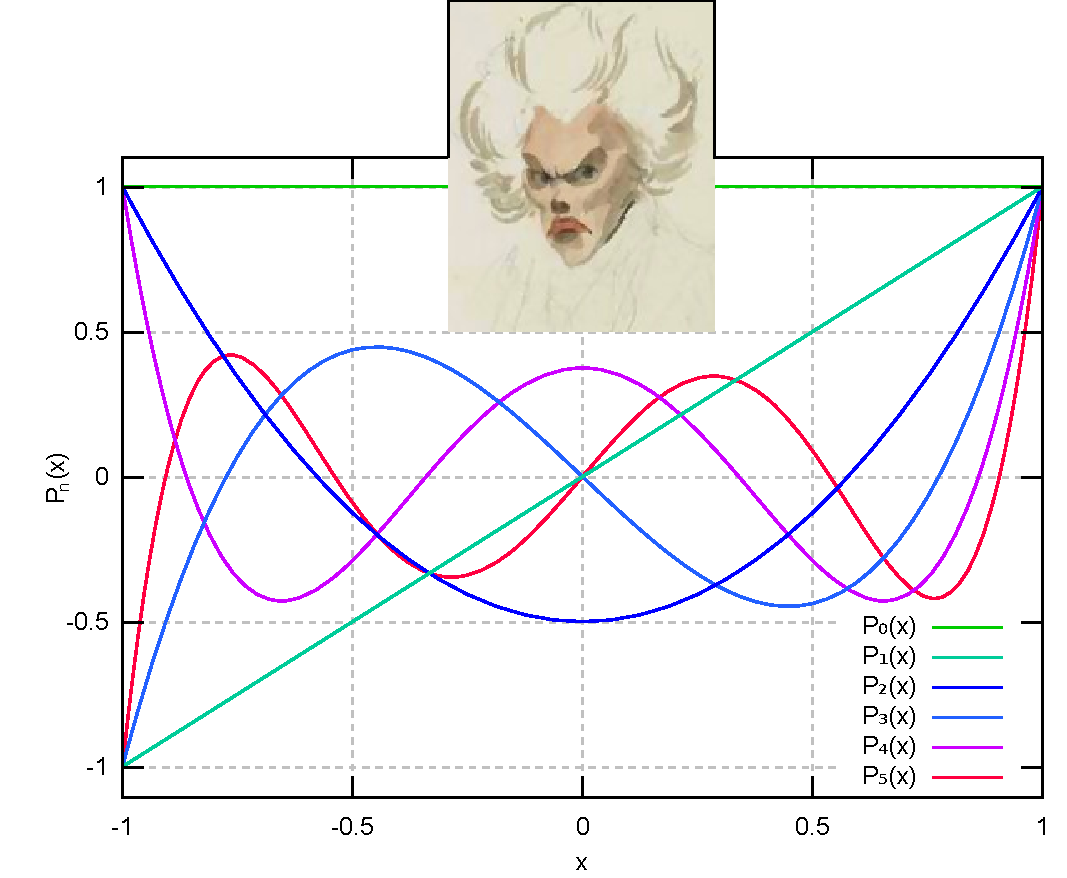
\includegraphics[height=.8\textheight]{obr/legendre}
  %\vspace{-1em}
  \begin{itemize}
  	\item \footnotesize $\P{0}(\mu) = 1,\ \ \P{1}(\mu) = \mu,\ \ \P{2}(\mu) = \frac12(3\mu^2 - 1),\ \ \P{2}(\mu) = \frac{1}{8} \left(3-30 \mu ^2+35 \mu ^4\right),\ \ \ldots$
  \end{itemize}
\end{frame}

\begin{frame}[t]
  \frametitle{Rozvoj do řady Legendreových polynomů}
  
  	  \centering$\Sigma_s(\br, \mu_0) = \suma[k]{0}{\infty}\frac{2k+1}{4\pi}\Sigma_{sk}(\br)\P{k}(\mu_0)$\\[.5em]
  	  
  \begin{itemize}	  
	  \item<2-> $\muint \P{j}(\mu)\P{k}(\mu) = \frac{2\delta_{jk}}{2k + 1}$\\[1em]
	  \item<2->[\Rabullet] $\Sigma_{sk}(\br) = 2\pi \muint[_0] \P{k}(\mu_0)\Sigma_s(\br, \mu_0)$
      \uncover<3->{\\[1em]
        $\Sigma_{s0}(\br) = \Sigma_s(\br)$\\[.5em]
   	    $\Sigma_{s1}(\br) = 2\pi \muint[_0] \mu_0\Sigma_s(\br, \mu_0)\uncover<4->{ = \muav(\br) \Sigma_s(\br)}$
   	    \begin{myitemize}
   	    	\item<4-> $ \muav(\br) = \frac{2\pi \muint[_0] \mu_0\Sigma_s(\br, \mu_0)}{2\pi \muint[_0] \Sigma_s(\br, \mu_0)} $~~\ldots~ 
   	    	\emph{střední kosinus rozptylových úhlů}\uncover<5>{\\[.5em]
   	    	$\big( = 2/(3A)$ pro elastický rozptyl na atomu s nukleonovým číslem $A\,\big)$}
   	    \end{myitemize}
   	}
  \end{itemize}

\begin{tikzpicture}[remember picture,overlay]  
  \node [xshift=-0.9cm,yshift=-1.1cm] at (current page.north east)
    {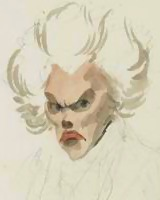
\includegraphics[width=1.5cm]{obr/Legendre.jpg}};
\end{tikzpicture}

\end{frame}

\begin{frame}
  \frametitle{Součtový vzorec}
\vspace{.75em}
\begin{overlayarea}{\textwidth}{\textheight}
\begin{itemize}
	\item Chceme vyjádřit
	  \alt<1-2>{
      $$
    	  (H\angflux)(\br,\alert<1-2>{\bomega}) = \aintp{
          \Sigma_s(\br, \bomega'\cdot\alert<1-2>{\bomega})
          \angflux(\br,\bomega')
        }
    	$$
   }{\\[1em]\hspace{1em}
      $
    	  (H\angflux)(\br,\alert<1-2>{\bomega}) = \aintp{
          \Sigma_s(\br, \bomega'\cdot\alert<1-2>{\bomega})
          \angflux(\br,\bomega')
        }
    	$
    	\vspace{0.75em}
   }
  \item<2-7> Zatím máme jen 
    \alt<1-2>{
      $$
        \Sigma_s(\br, \textcolor<2>{cyan}{\mu_0}) = \suma[k]{0}{\infty}\frac{2k+1}{4\pi}\Sigma_{sk}(\br)\P{k}(\textcolor<2>{cyan}{\mu_0})
      $$
      \vspace{-1.65em}
    }{\\[1em]\hspace{1em}
      $\Sigma_s(\br, \textcolor<2>{cyan}{\mu_0}) = \suma[k]{0}{\infty}\frac{2k+1}{4\pi}\Sigma_{sk}(\br)\P{k}(\textcolor<2>{cyan}{\mu_0})$
      \vspace{-.25em}
    }
    \alt<2-3>{
      \begin{align*}
	      \textcolor<2>{cyan}{\mu_0} &= \textcolor<2>{cyan}{\bomega'\cdot\bomega}
	      \uncover<3->{\\
      &= \lvect{\sint'\cosp',\sint'\sinp',\cost'}\!\cdot\!
	      \lvec{\sint\cosp,\sint\sinp,\cost}\\
      & = \mu'\mu + \sqrt{(1-\mu'^2)(1-\mu^2)}\cos(\azimuthal' - \azimuthal)\qquad\quad\qquad \big(\,\mu = \cos(\polar)\,\big)    
        }
      \end{align*}\vspace{-.5em}
    }{\\[1.25em] ale \vspace{-.25em}
      \begin{align*}
        \P{k}(\mu_0)
        &=P_k(\mu) P_k(\mu')+2 \sum _{m = 1}^k \frac{(k-m)!}{(k+m)!} \cos \bigl(m(\azimuthal - \azimuthal')\bigr) P_k^m(\mu) P_k^m(\mu')
        \uncover<5-7>{\\
        &=\frac{4\pi}{2k+1}\suma[m]{-k}{k}\textcolor<7>{blue}{\Y{k}{m}}(\alt<5>{\polar,\azimuthal}{\alert<6>{\bomega}})\textcolor<7>{blue}{\Yc{k}{m}}(\alt<5>{\polar',\azimuthal'}{\alert<6>{\bomega'}})
        }
      \end{align*}
    }
\end{itemize}
\end{overlayarea}

\begin{tikzpicture}[remember picture,overlay]  
  \alt<1-2>{
    \node [xshift=-0.9cm,yshift=-1.1cm] at (current page.north east)
      {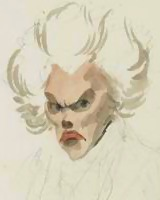
\includegraphics[width=1.5cm]{obr/Legendre.jpg}};
  }{
    \node [xshift=-2.7cm,yshift=-3cm] at (current page.north east)
      {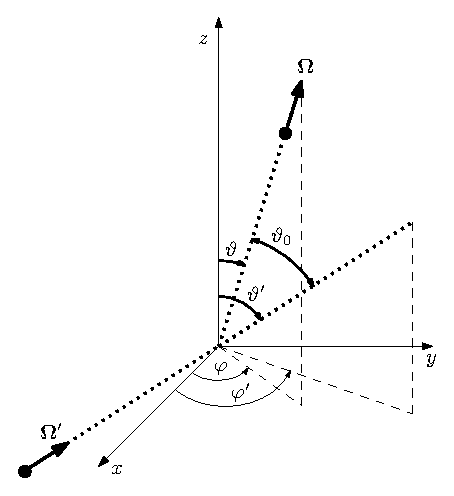
\includegraphics[width=5cm]{obr/scattering}};
  }
  \only<3->{
    \node [xshift=0.9cm,yshift=1.1cm] at (current page.south west)
      {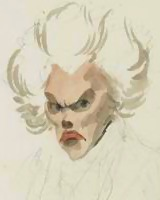
\includegraphics[width=1.5cm]{obr/Legendre.jpg}};
  }
\end{tikzpicture}

\end{frame}

\begin{frame}
  \frametitle{Sférické harmoniky}
  \framesubtitle{Definice}
  \begin{itemize}
  	\item<1-3> Sférická harmonická funkce \textcolor{structure}{\emph{řádu $m$}} a \textcolor{structure}{\emph{stupně $l$}}
  	  \begin{gather*}
        \Y{l}{m}(\bomega) = \Y{l}{m}(\alt<1>{\polar}{\mu},\azimuthal) = \sqrt{\frac{2l+1}{4\pi}\frac{(l-m)!}{(l+m)!}} \P{l}^m(
          \alt<1>{\cos\polar}{\mu}
        )e^{i m \azimuthal}\\[.5em]
        \alt<1>{\polar\in [0,\pi]}{\mu\in[-1,1]},\ \azimuthal\in [0,2\pi),\quad 
        l\in\mathbb{N}_0,\ m\in\mathbb{Z},\ 0\leq m \leq l
      \end{gather*}
    \item<3> \textcolor{structure}{\emph{Přidružené Legendreovy funkce}} (\emph{Associated Legendre functions})
    $$
      \P{l}^m(\mu) = 
      \begin{cases} 
        (-1)^m\sqrt{(1-\mu^2)^m}\ \der[m]{\P{l}(\mu)}{\mu} & \hphantom{-}\,0 \leq m \leq l,\\[1em]
        \displaystyle (-1)^{-m}\,\frac{(l+m)!}{(l-m)!}\P{l}^{-m}(\mu) & -l \leq m < 0 
      \end{cases}
    $$
  \end{itemize}
  
\begin{tikzpicture}[remember picture,overlay]  
  \node [xshift=-1cm,yshift=-0.8cm] at (current page.north east)
    {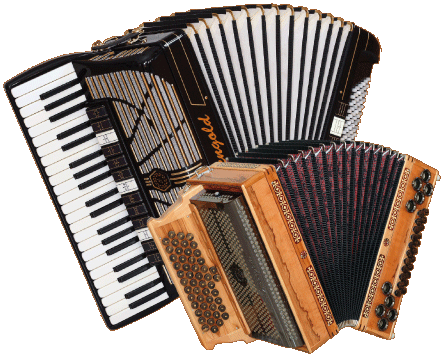
\includegraphics[width=1.75cm]{obr/harmoniky.png}};

   \only<4>{ 
     \node [anchor=center,yshift=-0.8cm] at (current page.center)
       {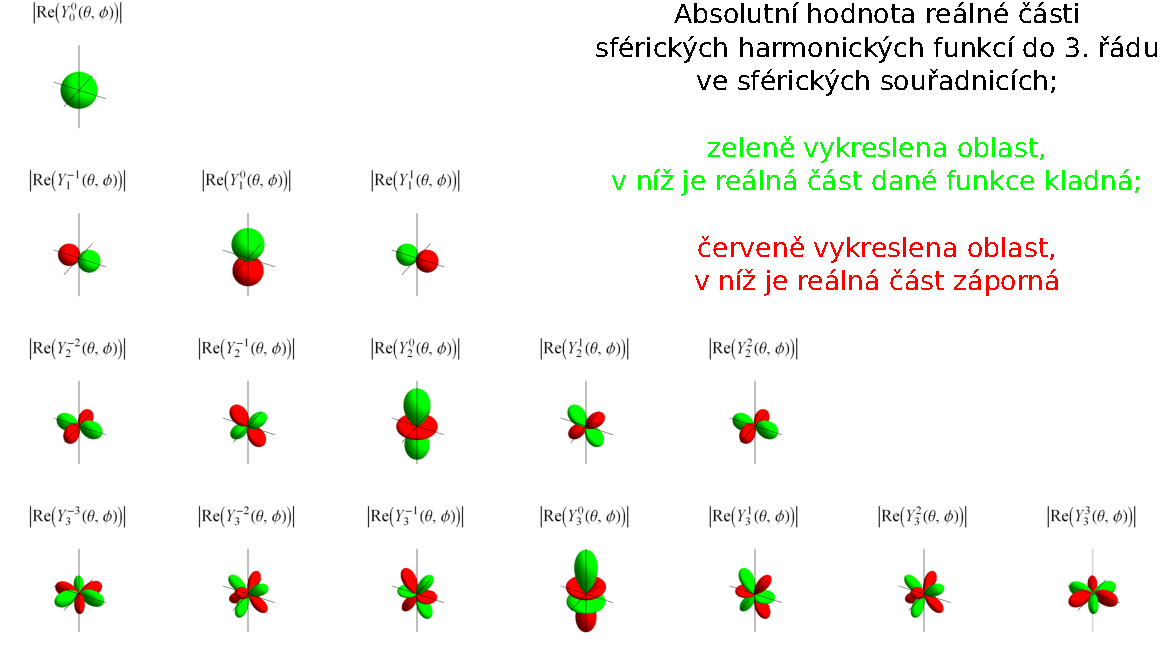
\includegraphics[width=1.05\textwidth]{obr/sh}};
   }
\end{tikzpicture}

\end{frame}

\begin{frame}
  \frametitle{Sférické harmonické funkce}
  \framesubtitle{Vlastnosti}
  \begin{itemize}
  	\item Úplný ortonormální systém na sféře vzhledem ke skalárnímu součinu
  	  $$
        \aint{\Y{l}{m}(\bomega)\Yc{l}{m}(\bomega)}
        = \int_{0}^{2\pi}\d{\azimuthal}\int_{-1}^{1}\d{\mu}
        \Y{l}{m}(\mu,\azimuthal)\Yc{l'}{m'}(\mu,\azimuthal)
      $$
    \item SHF stupně $l$ generují rotačně invariantní podprostor $\Lp{2}(\SS)$:
      $$\Lambda_l = \mathrm{Span}\bigl\{\Y{l}{m}; -l \leq m \leq l\bigr\},$$
    takový, že $R(\Lambda_l) \subset \Lambda_l$ pro libovolnou rotaci $R$
    \begin{itemize}
    	\item<2-> vlastní prostor příslušný $l$-tému vl. č. Laplaceova-Beltramiho
    operátoru $\nabla\cdot(\nabla)$ na sféře
      \item<3-> \alert{vlastní prostor libovolného rotačně invariantního operátoru}
    \end{itemize}
    
    \item<4-> Lze je použít pro zobecněný Fourierův rozvoj (tzv. \emph{Laplaceův rozvoj})
    funkcí def. na sféře -- 3D analogie rozvoje pomocí trigon. polynomů
    \item<5-> Azimutálně symetrické (nezávislé na $\azimuthal$ SHF: Legendreovy polynomy
   
  \end{itemize}
\end{frame}

\begin{frame}
  \frametitle{Sférické harmonické funkce}
  \framesubtitle{Použití -- reprezentace operátoru rozptylu}
  
  \begin{itemize}
  	\item Zobecněný Fourierův rozvoj rotačně invariantního operátoru rozptylu
  	do řady jeho vlastních funkcí
  \end{itemize}
\begin{align*}
\alert<6>{(H\angflux)(\br,\bomega)} &= 
  \aintp{
    \Sigma_s(\br, \bomega'\cdot\bomega)
    \angflux(\br,\bomega')
  }\uncover<2->{\\
& = \aintp{
      \suma[k]{0}{\infty}
        \frac{2k+1}{4\pi}\Sigma_{sk}(\br)\P{k}(\bomega'\cdot\bomega)
        \angflux(\br,\bomega')
    }\uncover<3->{\\
& = \aintp{
      \suma[k]{0}{\infty}
	      \Sigma_{sk}(\br)\suma[m]{-k}{k}\Y{k}{m}(\bomega)\Yc{k}{m}(\bomega')
        \angflux(\br,\bomega')
    }\uncover<4->{\\
& = \suma[k]{0}{\infty}
	    \Sigma_{sk}(\br)\suma[m]{-k}{k}\Y{k}{m}(\bomega) \aintp{
	      \Yc{k}{m}(\bomega')\angflux(\br,\bomega')
	    }\uncover<5->{\\
& \alert<6>{= \suma[k]{0}{\infty}
      \Sigma_{sk}(\br)\suma[m]{-k}{k}\Y{k}{m}(\bomega)\angmomgen{k}{m}(\br)}
}}}}
\end{align*}

\end{frame}

\begin{frame}
  \frametitle{Sférické harmonické funkce}
  \framesubtitle{Použití -- reprezentace operátoru rozptylu}
  
  \centering \alert<1>{$(H\angflux)(\br,\bomega) = \suma[k]{0}{\infty}\Sigma_{sk}(\br)\suma[m]{-k}{k}\Y{k}{m}(\bomega)\alert<2>{\angmomgen{k}{m}(\br)}$}
  
  \begin{itemize}
  	\item<2-> \alert<2>{$\angmomgen{k}{m}(\br) = \aint{\Yc{k}{m}(\bomega)\angflux(\br,\bomega)}$}\vspace{.5em}
  	\begin{itemize}
  		\item[\ldots]	  koeficienty zobecněného Fourierova rozvoje $\angflux(\br,\bomega)$ vzhledem k $\bomega$:
  		  \vspace{-.5em}
    		  \begin{equation*}
    		    \angflux(\br,\bomega) = \suma[k]{0}{\infty}\suma[m]{-k}{k}\angmomgen{k}{m}(\br)\Y{k}{m}(\bomega)
    		  \end{equation*}
   	\end{itemize}
    \item<3-> Finitní reprezentaci operátoru rozptylu získáme použitím konečného rozvoje ($0 \leq k \leq L < \infty$):
    \begin{myitemize}
    	\item rozptylovací charakteristiku každého materiálu uchováváme v podobě pole příslušných koeficientů $\Sigma_{sk}$
    \end{myitemize}
  \end{itemize}

\end{frame}

\begin{frame}
  \frametitle{Sférické harmonické funkce}
  \framesubtitle{Použití -- metoda $P_L$}
  
  \begin{itemize}
  	\item  Rozvoj 
  	  \begin{equation*}
		    \angflux(\br,\bomega) = \suma[k]{0}{L}\suma[m]{-k}{k}\angmomgen{k}{m}(\br)\Y{k}{m}(\bomega)
		  \end{equation*}
		  pro $L < \infty$ lze použít přímo k definici přibližného řešení LBR:
		  \begin{myitemize}
		  	\item dosazením rozvoje do LBR, použitím rozvoje operátoru rozptylu z předchozích slajdů a 
		  	  aplikací Galerkinovy metody vzhledem ke směrové proměnné získáme soustavu PDR 1. řádu 
		  	  v prostorové proměnné
		  	\item řešením vzniklé úlohy obdržíme $\angmomgen{k}{m}(\br)$, a tedy i $\angflux(\br,\bomega)$
		  \end{myitemize}
  \end{itemize}
  \uncover<2>{
\vspace{1em}
  \begin{center}
    {\huge  \textcolor{blue}{\emph{ O tom ale zas až někdy příště ...} ;-)}}
  \end{center}
  }
\end{frame}


%\begin{frame}[allowframebreak]
%%	\frametitle{Přehled}
% 	  \tableofcontents[part=1]
% 	  \vspace{-.5em}\tocrule\smallskip
% 	  \tableofcontents[part=2]
% 	  \vspace{-.5em}\tocrule\smallskip
%   	\tableofcontents[part=3]
%\end{frame}
%
%\part{Transportní rovnice neutronů}
%
%  \section{Předpoklady a definice}
%    \begin{frame}
  \frametitle{Základní předpoklady}
  
  \begin{itemize}
  	\item Neutrony lze popsat jako bodové objekty, ovlivněné pouze jadernými silami
  	\begin{itemize}
  		\item[\Rabullet] pohyb neutronů po přímých drahách
  		\item[\Rabullet] interakce s okolními atomy vede k záchytu či změně směru anebo rychlosti neutronu
  	\end{itemize}
  	\item Vzájemné interakce mezi neutrony jsou zanedbatelné
  	\item Izotropní prostředí, atomy sféricky symetrické
  	\begin{itemize}
  		\item samotný rozptyl a pohyb neutronů však může být anizotropní
  	\end{itemize}
  	\item Stacionární rozložení atomů (zanedbáváme tepelný pohyb)
  \end{itemize}

  \uncover<2->{
    \alert{Pohyb neutronů prostředím lze popsat lineární Boltzmannovou rovnicí}
    \begin{center}
    	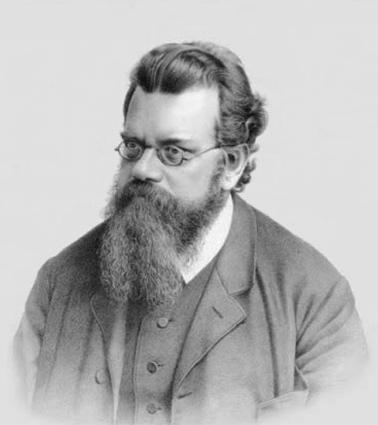
\includegraphics[scale=0.30]{obr/Boltzmann.jpg}
    \end{center}
  }
  
\end{frame}

\begin{frame}[t]
  \frametitle{Stavový prostor}
 
  $$
    X = \VV \times \EE \times \SS \equiv \{x = (\br,E,\bomega):\ \br\in \VV, E \in \EE, \bomega\in \SS\}
  $$
  
  \begin{center}
	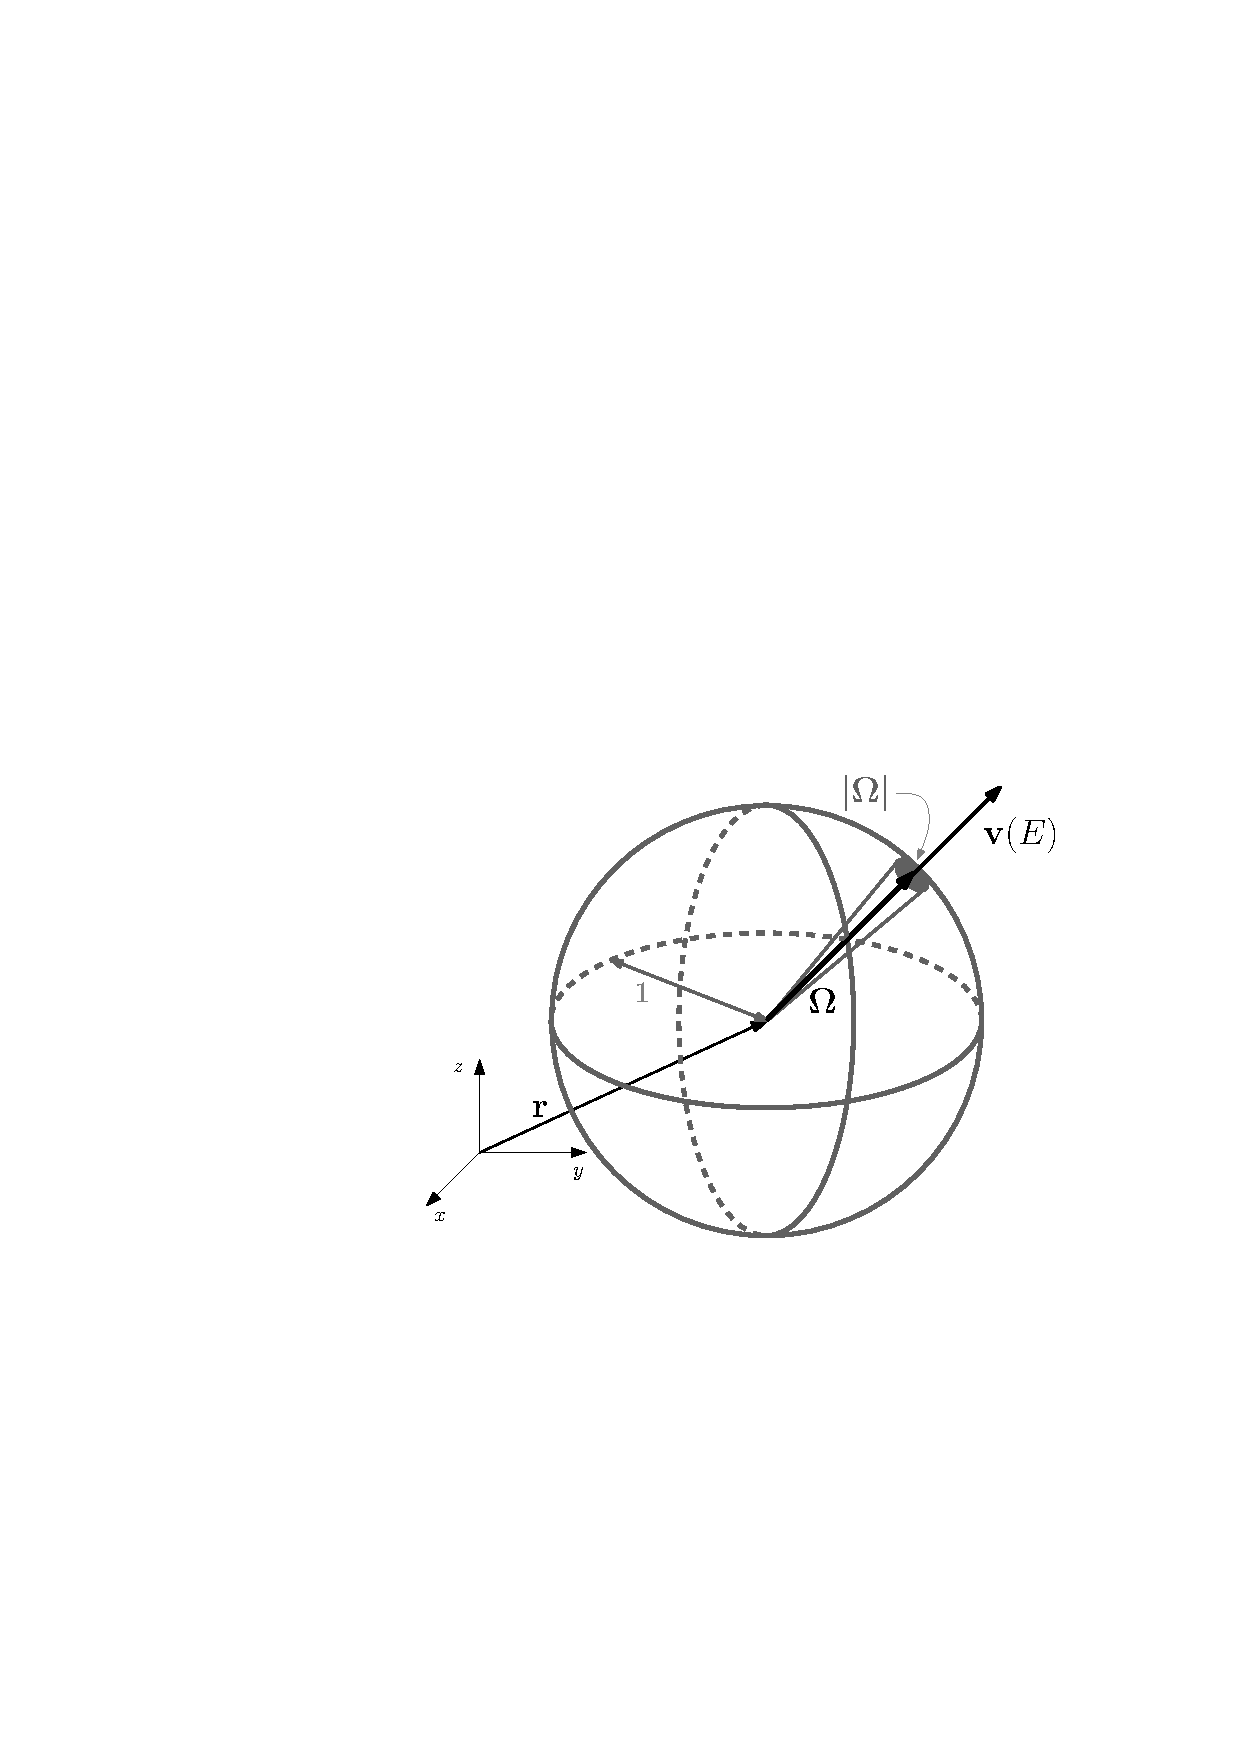
\includegraphics[scale=0.70]{obr/stavovy_prostor}\\[1em]
	\alert{6 dimenzí}
  \end{center}

\end{frame}

\begin{frame}[t]
  \frametitle{Stavový prostor}
  \framesubtitle{Poloha}
 
  $$
    X = \VV \times \EE \times \SS \equiv \{x = (\alert\br,E,\bomega):\ \alert{\br\in \VV}, E \in \EE, \bomega\in \SS\}
  $$
  
  \begin{columns}
  \column{.5\textwidth}
    \centering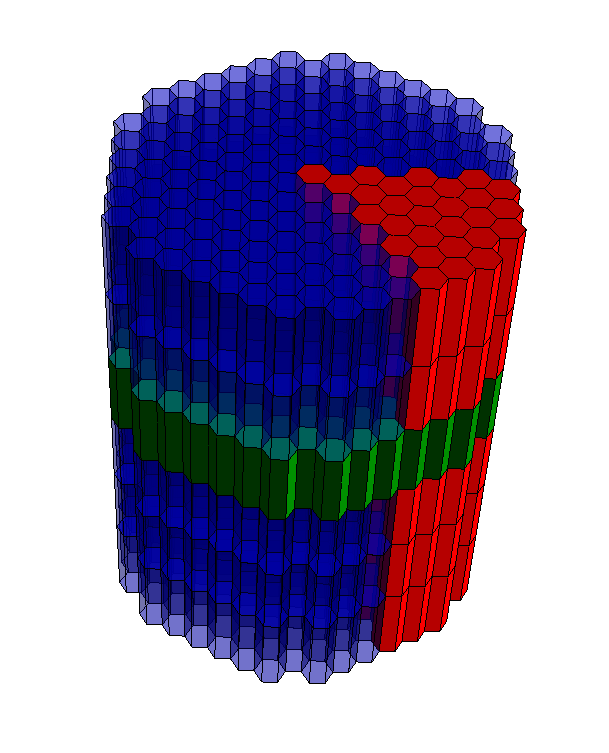
\includegraphics[scale=0.225]{obr/core.png}
  \column{.5\textwidth}
    \includegraphics<1>[scale=0.425]{obr/core/core_level1}
	  \includegraphics<2>[scale=0.425]{obr/core/core_level2}
	  \includegraphics<3>[scale=0.425]{obr/core/core_level3}
	  \includegraphics<4>[scale=0.425]{obr/core/core_level4}
	  \includegraphics<5>[scale=0.425]{obr/core/core_level5}
	  \includegraphics<6>[scale=0.425]{obr/core/core_level6}
	  \includegraphics<7>[scale=0.425]{obr/core/core_level7}
	  \includegraphics<8>[scale=0.425]{obr/core/core_level8}
	  \includegraphics<9>[scale=0.425]{obr/core/core_level9}
	  \includegraphics<10>[scale=0.425]{obr/core/core_level10}
	  \transduration<1-9>{0.5}
	  \transduration<10>{500}    
  \end{columns}
  \hfill\alert{3 dimenze}\hfill\hbox{}
\end{frame}

\begin{frame}[t]
  \frametitle{Stavový prostor}
  \framesubtitle{Energie}
 
  $$
    X = \VV \times \EE \times \SS \equiv \{x = (\br,\alert E,\bomega):\ \br\in \VV, \alert{E \in \EE}, \bomega\in \SS\}
  $$
  \vspace{.5em}
  \begin{columns}
  \column{.5\textwidth}
  \centering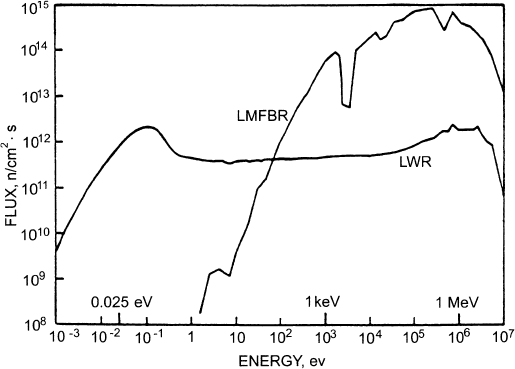
\includegraphics[width=.9\textwidth]{obr/spektrum}
  \column{.5\textwidth}
  \centering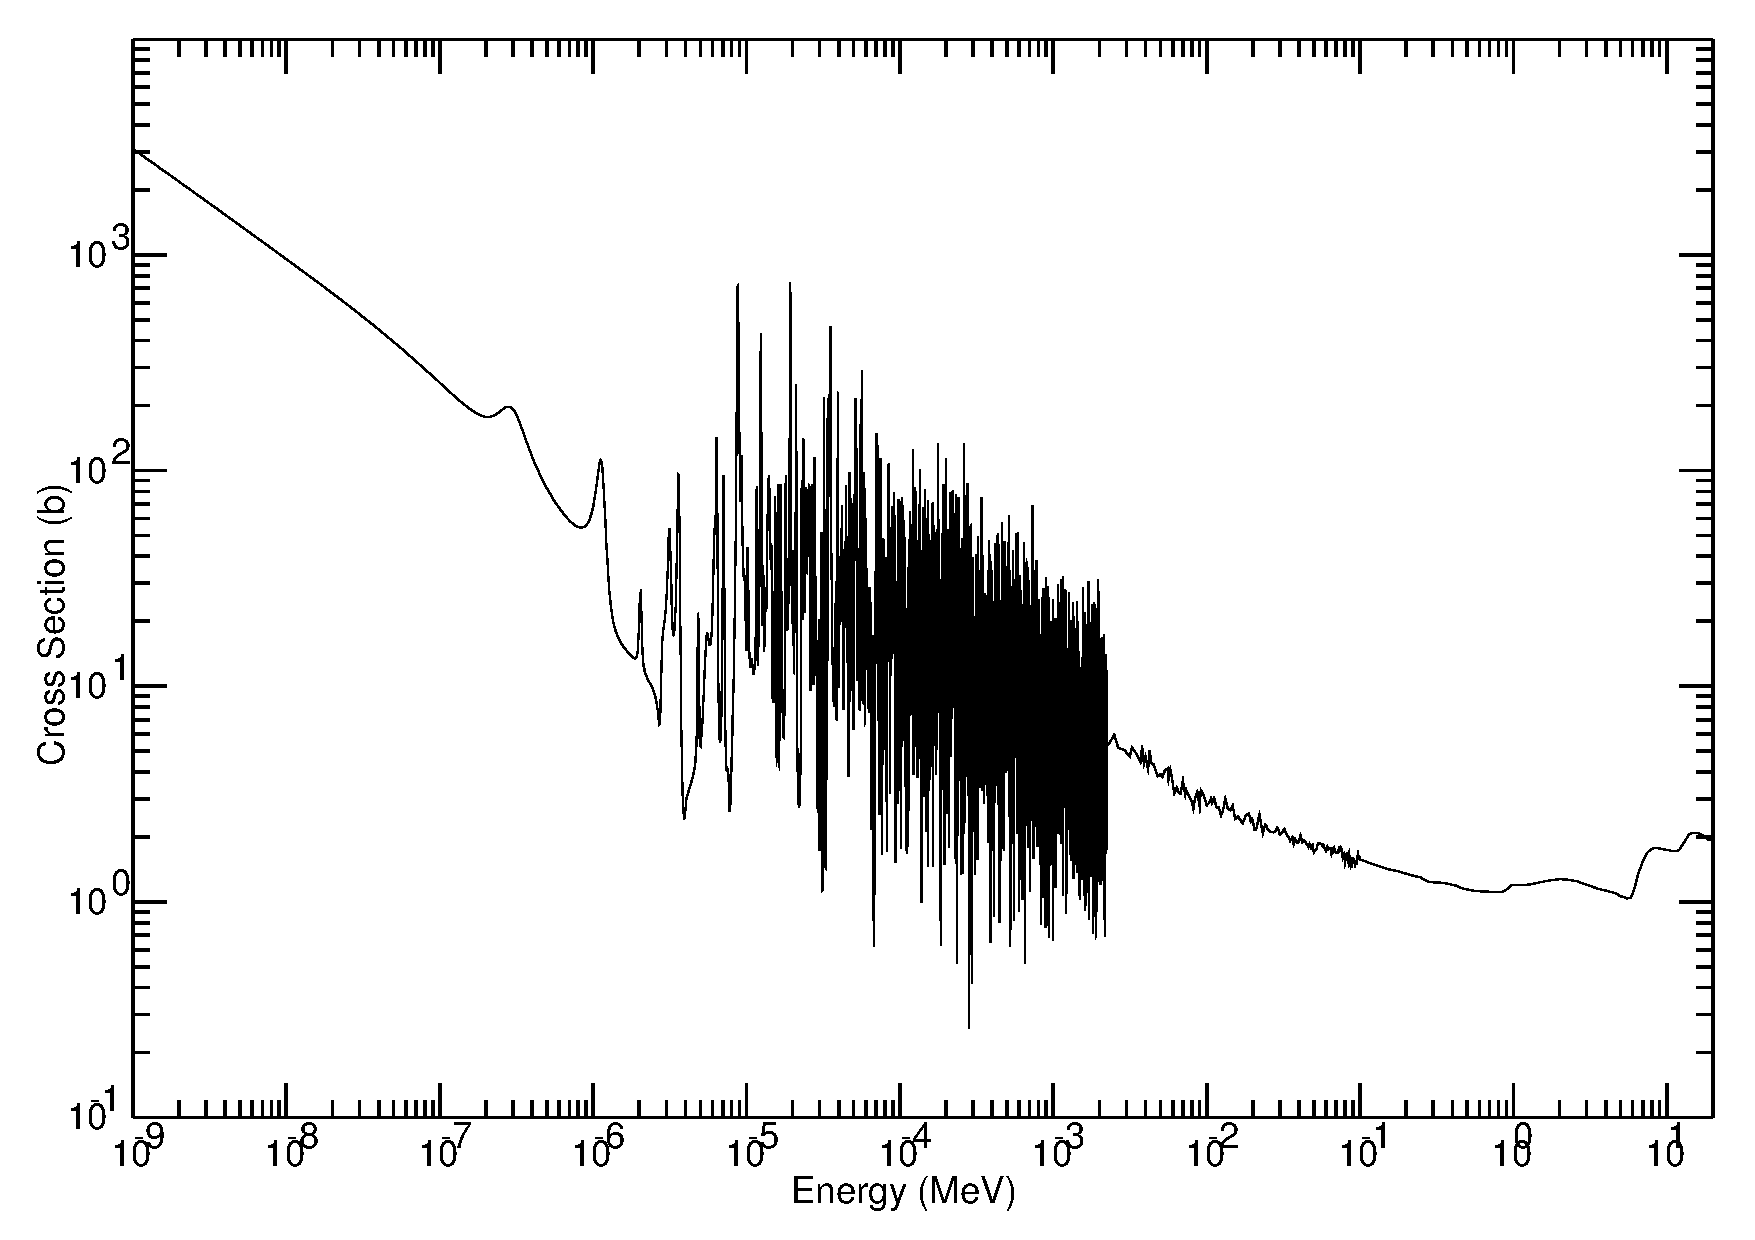
\includegraphics[width=.9\textwidth]{obr/U235f}
  \end{columns}
  \begin{center}
  \alert{1 dimenze}
  \end{center}
\end{frame}

\begin{frame}[t]
  \frametitle{Stavový prostor}
  \framesubtitle{Směr}
 
  $$
    X = \VV \times \EE \times \SS \equiv \{x = (\br,E,\alert\bomega):\ \br\in \VV, E \in \EE, \alert{\bomega\in \SS}\}
  $$
  
  
  \vspace{.5em}
  \begin{columns}
  \column{.5\textwidth}
  \centering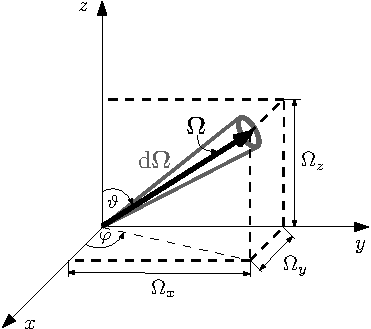
\includegraphics[width=.9\textwidth]{obr/cartesian_streaming}
  \column{.5\textwidth}
  \centering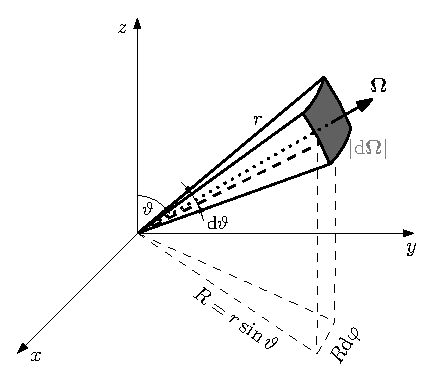
\includegraphics[width=.9\textwidth]{obr/element}
  \end{columns}
  \begin{center}
  \alert{2 dimenze}
  \end{center}
  
\end{frame}

\begin{frame}
  \frametitle{Základní směrově závislé veličiny}

  \begin{columns}[c]
  \begin{column}{.60\linewidth}  
    \begin{itemize}
    \item Hustota neutronů (v $\d{\br}\d{E}\d{\bomega}$):
    \begin{myitemize}
    	\item $N(\br,E,\bomega,t)$
    \end{myitemize}
  \end{itemize}
  \end{column}
  \begin{column}{.30\linewidth}  
  \end{column}
  \end{columns}
  
  \begin{columns}[c]
  \begin{column}{.60\linewidth}
  \begin{itemize}
	  \item Směrový neutronový tok
	  \begin{myitemize}
	    \item $\angflux(\br,E,\bomega,t) = v(E)N(\br,E,\bomega,t)$
	  	\item $\angflux(\br,E,\bomega,t)\,\d{\bomega}\d{E}$
	  \end{myitemize}
  \end{itemize}
  \end{column}
  \begin{column}{.30\linewidth}
  	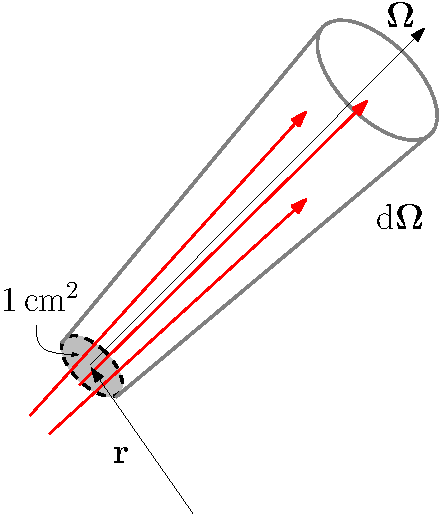
\includegraphics[scale=.45]{obr/angflux}
	\end{column}
	\end{columns}
	\vspace{-2em}
	\begin{columns}
	\begin{column}{.60\linewidth}
	\begin{itemize}
	  \item Směrový neutronový proud
	  \begin{myitemize}
	    \item $\bj(\br,E,\bomega,t) = \bomega \angflux(\br,E,\bomega,t)$\\
	  	\item $j(\br,E,\bomega,t) = \bn\cdot\bj(\br,E,\bomega,t)\,\d{S}\d{\bomega}\d{E}$
	  \end{myitemize}
  \end{itemize}
  \end{column}
  \begin{column}{.30\linewidth}
   	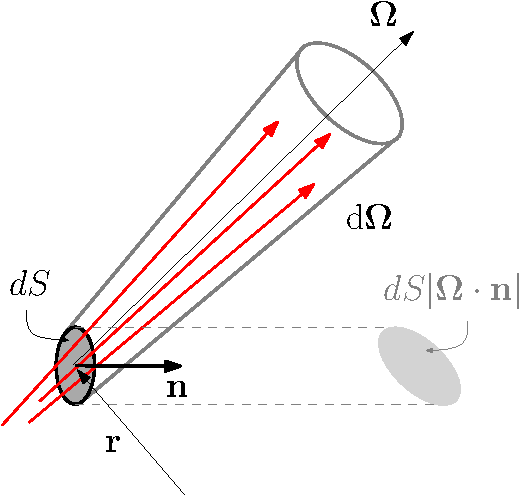
\includegraphics[scale=.45]{obr/angcur}
  \end{column}
  \end{columns}
\end{frame}

\begin{frame}
  \frametitle{Směrově nezávislé veličiny}
  \shorten{-.2em}{-.2em}
  \begin{itemize}
	  \item Skalární neutronový tok:
	    $$ \fl(\br,E,t) = \aint{\angflux(\br,E,\bomega,t)} $$
	  \item Úhrnný neutronový proud: 
	    $$\bJ(\br,E,t)	= \aint{\bj(\br,E,\bomega,t)} = \aint\bomega\angflux(\br,E,\bomega,t)$$
	  \item Parciální neutronový proud:
	    $$
	      j^{\pm}(\br,E,t) = \Aint[\bomega\cdot\bn \gtrless 0]{\abs{\bomega\cdot\bn}\angflux(\br,E,\bomega,t)}
	    $$
	    \vspace*{-.5em}
	  \begin{itemize}
	  	\item přestup neutronů
	  	  $\left.\begin{cases} \mbox{ve směru} &(j^+)\\
	  	    \mbox{proti směru} &(j^-)
	  	    \end{cases}\right\}$
	  	  vnější normály dané plochy
	  \end{itemize}
	  \vspace*{.5em}
	  \item Úhrnný neutronový proud (skalár): $j = \bJ\cdot\bn = j^+-j^-$
  \end{itemize}
\lengthen
\end{frame}

\begin{frame}
  \frametitle{Charakterizace interakcí}
    \begin{myitemize}
	  \item $\Sigma_t = \Sigma_a + \Sigma_f + \Sigma_s$
	  \begin{myitemize}
	  	\item funkce $\br$, $E$, $t$, ale ne $\bomega$ (izotropní prostředí -- stejné vlastnosti ve všech směrech)
	  \end{myitemize}
    \item Četnosti reakcí v objemu $\VV$ za časovou jednotku
	  \begin{myitemize}
	  	\item $\vint{\eint{\Sigma_{t,a,f,s}(\br,E,t)\fl(\br,E,t)}}$
	  \end{myitemize}
	  \item Změna energie a směru pohybu: $\chi(E'\ra E,\, \bomega'\ra\bomega)$
	  \begin{myitemize}
	  	\item štěpení -- \alert<2>{izotropní proces} v \alert<3>{izotropním prostředí}
	  	\begin{itemize}\vspace*{.25em}
	  		\item $\chi(E'\ra E, \alert<3>{\bomega'}\ra\alert<2>{\bomega}) = \alert<2>{\frac{1}{4\pi}}\chi_f(E'\ra E\alert<3>)$
	  	\end{itemize}
	  	\item rozptyl -- \alert<4>{anizotropní proces v izotropním prostředí}
	  	\begin{itemize}\vspace*{.25em}
	  		\item $\chi(E'\ra E, \alert<4>{\bomega'\ra\bomega}) = \chi_s(E'\ra E,\,\alert<4>{\bomega'\cdot\bomega})$
	  	\end{itemize}	  	
	  \end{myitemize}
  \end{myitemize}

\end{frame}



%    % zmínit křivočaré souřadnice
%  \section{Bilance směrového neutronového toku}
%    \begin{frame}[t]
  \frametitle{Bilance směrového neutronového toku}

  \alert<3>{Časová změna množství neutronů v elementu stavového prostoru $=$}
  \begin{itemize}
	  \item[$+$] \alert<4>{množství nově se objevivších neutronů}
	  \item[$-$] \alert<5>{množství zachycených neutronů}
	  \item[$-$] \alert<6>{množství neutronů uniklých přes hranici}
  \end{itemize}
  
  \uncover<2->{
    \vspace{1em}
    Pomocí $\angflux$, u nějž předpokládáme
    \begin{itemize}
    	\item spojitou diferencovatelnost vzhledem k $t$\uncover<7->{, $\br$}
    \end{itemize}
    \shorten{-.4em}{0em}
    \alt<1-9>{
    \begin{multline*}
      {\color<3>{red}\Vint{\Eint{\Aint{\frac{1}{v(E)}\pd{\angflux(\br,E,\bomega,t)}{t}}}}} = 
      {\color<4>{red}\Vint{\Eint{\Aint{P(\br,E,\bomega,t)}}}}\\
      - {\color<5>{red}\Vint{\Eint{\Aint{\Sigma_t(\br,E,\bomega,t)\angflux(\br,E,\bomega,t)}}}}\\
      - \alt<1-6>{
          {\color<6>{red}\int_{\bnd}\Eint{\Aint{\bj(\br,E,\bomega,t)\bn(\br)\d{S}}}}
        }{
          \alt<7>{
            \Vint{\Eint{\Aint{\nabla\cdot\bj(\br,E,\bomega,t)}}}
          }{
            \Vint{\Eint{\Aint{\bomega\cdot\nabla\angflux(\br,E,\bomega,t)}}}
          }
        }
     \end{multline*}
     }{
     \begin{align*}
      \frac{1}{v(E)}\pd{\angflux(\br,E,\bomega,t)}{t} &=
      P(\br,E,\bomega,t)\\[-.25em]
      &- \Sigma_t(\br,E,\bomega,t)\angflux(\br,E,\bomega,t)\\[.4em]
      &- \bomega\cdot\nabla\angflux(\br,E,\bomega,t)
      \end{align*}
     }
    \lengthen
    \uncover<8-10>{ \alt<8-9>{($\bomega$ nezávisí na $\br$ \only<9>{-- \alert{ale jen v kartézských souřadnicích!}})}{($\d{\br}\d{E}\d{\bomega}$ libovolné)} }
  }
\end{frame}

\begin{frame}
  \frametitle{Bilance směrového neutronového toku}
  \framesubtitle{Zdrojový člen}
    \shorten{-.35em}{-.35em}
    \begin{multline*}
    \frac{1}{v(E)} {\pd{\angflux(\br,E,\bomega,t)}{t}} = \\
    {\alert<2-3>{P(\br,E,\bomega,t)}}
    - {\Sigma_t(\br,E,\bomega,t)\angflux(\br,E,\bomega,t)}
    - {\bomega\cdot\nabla\angflux(\br,E,\bomega,t)}
    \end{multline*}
    \pause
    \temporal<3>{
      \begin{align*}
        {\alert{P(\br,E,\bomega,t)}} &= 
          \aintp{\eintp{\nu\Sigma_{\color{cyan}{f}}(\br,E',t)\chi_{\color{cyan}{f}}(E'\ra E,\, \bomega'\ra\bomega)\angflux(\br,E',\bomega',t)}}\\
          &+
          \aintp{\eintp{\Sigma_{\color{magenta}{s}}(\br,E',t)\chi_{\color{magenta}{s}}(E'\ra E,\, \bomega'\ra\bomega)\angflux(\br,E',\bomega',t)}}\\[.25em]
          &+
          {Q(\br,E,\bomega,t)}
      \end{align*}
    }{
      \begin{align*}   
        {\alert{P(\br,E,\bomega,t)}} &= 
          \frac{1}{4\pi}\eintp{\nu\Sigma_{\color{black}{f}}(\br,E',t)\chi_{\color{black}{f}}(E'\ra E){\color{black}\fl(\br,E',t)}}\\
          &+
          \aintp{\eintp{\Sigma_{\color{black}{s}}(\br,E',t)\chi_{\color{black}{s}}(E'\ra E,\, \bomega'\cdot\bomega)\angflux(\br,E',\bomega',t)}}\\[.25em]
          &+
          {Q(\br,E,\bomega,t)}
      \end{align*}
    }{
      \begin{align*}   
        {P(\br,E,\bomega,t)} &= 
          \frac{1}{4\pi}\eintp{{\color{red}
            \alt<4>{
              \nu\Sigma_f(\br,E',t)\chi_f(E'\ra E)
             }{
              \nu\Sigma_f(\br,E'\ra E,t)
             }}\fl(\br,E',t)}\\
          &+
          \aintp{\eintp{{\color{red}
            \alt<4>{
              \Sigma_s(\br,E',t)\chi_s(E'\ra E,\, \bomega'\cdot\bomega)
            }{
              \Sigma_s(\br,E'\ra E,\, \bomega'\cdot\bomega,t)
            }}\angflux(\br,E',\bomega',t)}}\\[.25em]
          &+
          {Q(\br,E,\bomega,t)}
      \end{align*}
    }   
    \lengthen
    \vspace*{-.4em}
    \uncover<3-5>{
      \begin{itemize}
      	\item předpoklady na izotropii
      	\item veškeré štěpení pro jednoduchost okamžité, bez zpožděných neutronů
      \end{itemize} 
    }     
\end{frame}


\begin{frame}
  \frametitle{Doplňující předpoklady a podmínky}
  \begin{itemize}
  	\item Pro skoro všechna $x\in X$: 
  	$$
  	\begin{gathered}
	    \begin{array}{ccl}
	    0 \leq& \!\!\!\Sigma_t(x,t)\!\!\! &< \infty,\\
	    0 \leq& \!\!\!\angflux(x,t)\!\!\! &< \infty,\\
	    0 \leq& \!\!\!Q(x,t)\!\!\! &< \infty,
	    \end{array}\\
	    \Sigma_t,\, \angflux\, \not\equiv 0.
	    \end{gathered}
    $$
    \item $\Sigma_t(\cdot,t)\in L^{\infty}(X)$,~ $\angflux(\cdot,t),\, Q(\cdot,t)\, \in \Lp{1}(X)$\vspace{.5em}
    \item $\aint{\eint{\chi_{s,f}(E'\ra E, \bomega'\ra \bomega)}} = 1$\vspace{.5em}
    \item Počáteční podmínka: $\angflux(\br,E,\bomega,t_0) = \Psi_0(\br,E,\bomega)$\vspace{.5em}
    \item Okrajové podmínky na \emph{\color{structure}vtokové hranici}
  \end{itemize}
  
  
\end{frame}

\begin{frame}
  \frametitle{Okrajové podmínky}
  \framesubtitle{Pomocné definice}
  
  \begin{itemize}
  	\item Homogenní / nehomogenní hranice: $\pV = \pVn \cap \pVh$
  	\hspace*{-3em}
  	\begin{minipage}{\paperwidth}
    $$
      \angflux_{\mathrm{in}}(\br,E,\bomega,t) = \begin{cases}
      \Psi_{\mathrm{in}}(\br,E,\bomega,t)\\
      0
      \end{cases}\hspace{-1em},\
      \angflux_h(\br,E,\bomega,t) = \begin{cases}
      0 & \br\in\pVn\\
      \Psi_h(\br,E,\bomega,t) & \br\in\pVh
      \end{cases}
    $$
    \end{minipage}\vspace{.75em}
    \item Vtoková / odtoková hranice:
  	$$
      \only<1>{\pX[\pm]}\only<2>{\pX[\pm]_{\;\color{red}0}}\only<3>{\pX[\pm]_{\,\color{red}h}} = 
        \bigl\{
          x = ({\color{cyan}\br}, {\color{magenta}E}, {\color{dkgreen}\bomega)}:
          {\color{cyan}\br \in \only<1>{\pV}\only<2>{\pV_{\color{red}0}}\only<3>{\pV_{\color{red}h}}},\ 
          {\color{magenta} E \in \EE},\ 
          {\color{dkgreen}\bomega\in\SS\land\bomega\cdot\bn(\br) \gtrless 0}
        \bigr\}
    $$
    \item Úhel zrcadlového odrazu (\emph{specular reflection}):
    \shorten{-.1em}{-1.5em}
    $$
      \bomega_R = \bomega - 2 \bn (\bomega \cdot \bn)
    $$
    \lengthen
    \begin{itemize}
    	\item Householderova transf. vektoru $\bomega$ vzhledem k rovině s normálou $\bn$
    	\item Úhel odrazu $=$ úhel dopadu:  $\abs{\bomega\cdot\bn} = \abs{\bomega_R\cdot\bn}$
    	\item Úhel odrazu leží ve stejné rovině jako úhel dopadu: $(\bomega_R\times\bn)\cdot\bn = 0$
    \end{itemize}
    
  \end{itemize}

\end{frame}

\begin{frame}
  \frametitle{Okrajové podmínky}
  \framesubtitle{Vybrané typy}
  $$
    \angflux(x,t) = \angflux_{\mathrm{in}}(x,t) + \alert<2->{\angflux_h(x,t)},\quad x = (\br,E,\bomega)\in\pX
  $$
  \pause
  \begin{itemize}
  	\item<3-> \alt<3>{Nonreentrantní}{Volná} hranice\uncover<5->{
  	-- rozhranní mezi zkoumaným prostředím a
    vakuem, příp. perfektním absorbérem (\emph{black body})
  	$$
  	  \angflux_h(x,t) = 0,\quad x\in\pX[-]_h
  	  \qquad (\Longrightarrow\ \ j^{-}(\br,E,t) = 0)
  	$$
  	}    
  	\item<6-> Zrcadlový odraz (\emph{specular reflection})
  	$$
  	  \angflux_h(x,t) = \angflux(\br,E,\bomega_R,t),\quad x\in\pX[-]_h
  	$$
  \end{itemize}

\end{frame}

\begin{frame}
  \frametitle{Okrajové podmínky}
  \framesubtitle{Vybrané typy}
  \shorten{-.5em}{-1em}
  $$
    \angflux(x,t) = \angflux_{\mathrm{in}}(x,t) + \alert<1-2>{\angflux_h(x,t)},\quad x = (\br,E,\bomega)\in\pX
  $$
  \lengthen
  \begin{itemize}
  	\item Okrajová podmínka typu albedo
  	$$
  	  \angflux_h(x,t) = \bndint[']{\pX[+]_h}\beta(x'\ra x,t)\angflux(x',t),\quad x\in\pX[-]_h,
  	$$
  	kde $\db{x'} = \abs{\bomega'\cdot\bn}\d{S}\d{E'}\d{\bomega'}$
  	
  	\uncover<2->{
  	\begin{myitemize}
  	 	\item $\beta$ charakterizuje případy, kdy v okamžiku $t$ neutron opouští prostředí\\
  	 	  v místě $\br'$, s energií $E'$ a ve směru $\bomega'$ a jiný neutron se vrací\\
  	 	  v jiném místě $\br$, s jinou energií $E$ a v jiném směru $\bomega$.
      \item Jiné typy podmínek lze získat lokalizací, např. zrcadlový odraz:\\[.3em]\centering 
        $\beta(\br'\ra \br, E'\ra E, \bomega'\ra\bomega,t) = \delta(\br' - \br)\delta(\bomega' - \bomega_R)\delta(E' - E)$
  	 \end{myitemize}\vspace{.2em}
  	}
  	\item<3-> Spojitost směrového toku na vnitřních rozhranních ($\forall E,\ \bomega$)
  \end{itemize}

\end{frame}

%TODO: White B.C, isotropic reflection, source condition


%    % zmínit zpožděné neutrony
%  \section{Různé podoby}
%    \begin{frame}
  \frametitle{Ustálený stav}
  
    \begin{multline*}
    \frac{1}{v(E)} {\pd{\angflux(\br,E,\bomega,t)}{t}} = \\
    {P(\br,E,\bomega,t)}
    - {\Sigma_t(\br,E,\bomega,t)\angflux(\br,E,\bomega,t)}
    - {\bomega\cdot\nabla\angflux(\br,E,\bomega,t)}
    \end{multline*}
    + počáteční a okrajové podmínky
    \uncover<2>{
    \begin{center}
    \begin{tikzpicture}
      \draw[decorate, decoration=snake,thick,structure,->] (0,0) -- (0,-1);
    \end{tikzpicture}
    \end{center}
    $$
      \bomega\cdot\nabla\angflux(\br,E,\bomega) +
      \Sigma_t(\br,E,\bomega)\angflux(\br,E,\bomega) =
      P(\br,E,\bomega)
    $$
    \\[.5em]
    + okrajové podmínky
    }

\end{frame}

\begin{frame}
  \frametitle{Operátorový zápis}
  \framesubtitle{integro-diferenciální LBR}
  
$$
  \left\{
    \begin{aligned}
       \alert<2-3>{L\angflux} &= P \equiv \alert<4>{H\angflux} + \alert<5>{F\angflux} + \alert<6>{Q}\quad &&\mbox{ v $X$,}\\
	  \angflux  &= \alert<7>{\beta\angflux} + \angfluxin\quad   &&\mbox{ na $\pX[-]$.}
    \end{aligned}
  \right.
$$
\begin{itemize}
	\item<2-> \alert<2>{advekce} a \alert<3>{záchyt}: $(\alert<2-3>{L\angflux})(x) = \alert<2>{\bomega\cdot\nabla\angflux(x)} + \alert<3>{\Sigma_t\angflux(x)}$
	\item<4-> \alert<4>{rozptyl} a \alert<5>{stěpení}: 
	    \begin{align*}
		      (\alert<4>{H\angflux})(x) &= \aintp{\eintp{\Sigma_s(\br, E'\ra E, \bomega'\cdot\bomega)\angflux(\br,E',\bomega')}}\\
		      (\alert<5>{F\angflux})(x) &= \frac{1}{4\pi}\eintp{\nu\Sigma_f(\br, E'\ra E)\aintp{\angflux(\br,E',\bomega')}}
      \end{align*}
	\item<6-> \alert<6>{stálý vnější neutronový zdroj:} $\alert<6>{Q(x)}$
	\item<7-> \alert<7>{přestup přes okraje:}
	$$
		(\alert<7>{\beta\angflux})(x) = \bndint[']{\pX[+]}\beta(\br'\ra \br, E'\ra E, \bomega'\ra\bomega)\angflux(\br', E', \bomega')
  $$
\end{itemize}

\end{frame}

\begin{frame}
  \frametitle{Úloha na $\keff$}
  
  $$
  \left\{
    \begin{aligned}
       (L-H)\angflux &= \frac{1}{\keff} F\angflux &&\mbox{ v $X$,}\\
	  \angflux  &= \beta\angflux \quad   &&\mbox{ na $\pX[-]$.}
    \end{aligned}
  \right.
$$

\end{frame}

\begin{frame}
  \frametitle{Mnohagrupová integro-diferenciální LBR}
  
  \vspace{-1.25em}
  
  \hbox{}\hfill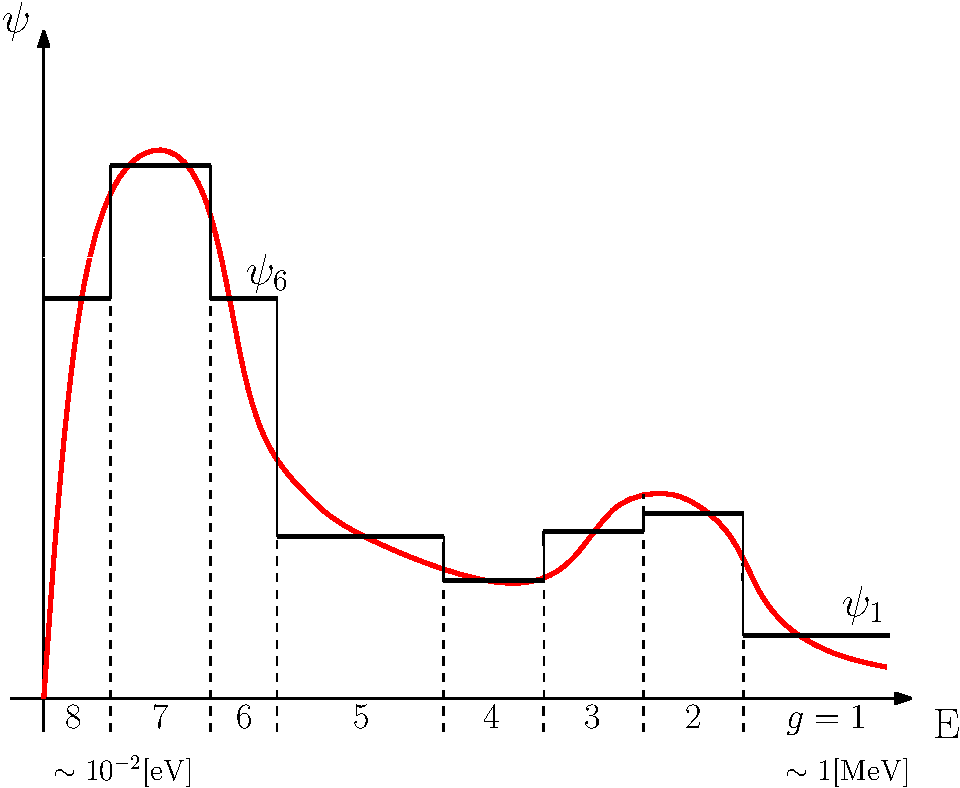
\includegraphics[width=.425\textwidth]{obr/fluxg}\hfill
  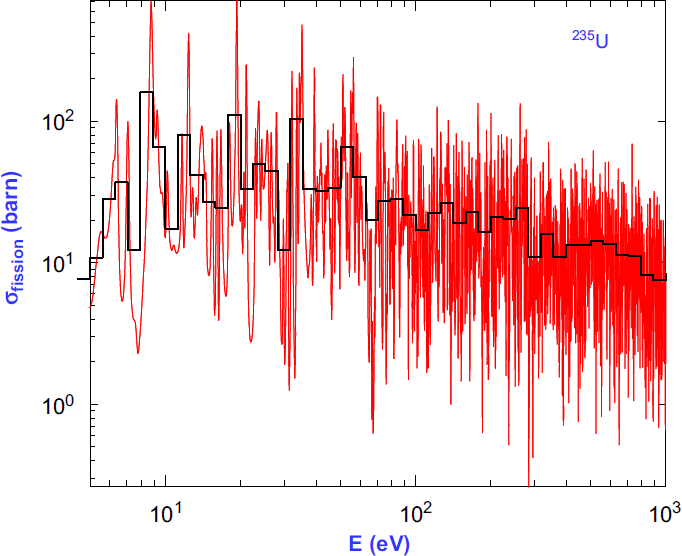
\includegraphics[width=.425\textwidth]{obr/U235fg}\hfill\hbox{}
  
  \shorten{-.6em}{0em}

  $$
  \left\{
    \begin{aligned}
    \llop\vangflux &= \hhop\vangflux + \ffop\vangflux + \QQ\quad &&\mbox{ v $X$,}\\
    \vangflux  &= \valbedo\vangflux + \vangflux_{\mathrm{in}}\quad   &&\mbox{ na $\pX[-]$}.
  \end{aligned}
  \right.
  $$

  \begin{gather*}
    \vangflux = \big[\angflux_g\big]_{g=1,\ldots, G}\quad
    \vangflux_{\mathrm{in}} = \big[\angflux_{\mathrm{in},g}\big]_{g=1,\ldots, G}\quad
    \QQ = \big[Q_g\big]_{g=1,\ldots, G}\\[.3em] 
    \llop = \big\llbracket L_{gg} \big\rrbracket_{g=1,\ldots, G} \\[.2em]
    \hhop = \big\llbracket H_{gg'}\big\rrbracket_{g,g'=1,\ldots, G} \quad
    \ffop = \big\llbracket F_{gg'}\big\rrbracket_{g,g'=1,\ldots, G} \quad
    \valbedo = \big\llbracket \beta_{gg'}\big\rrbracket_{g,g'=1,\ldots, G}
  \end{gather*}
  
  \lengthen
    
\end{frame}

\begin{frame}
  \frametitle{Monoenergetická podoba}
  
\begin{itemize}
	\item $ G = 1$,~ $\angflux = \angflux(\br,\bomega)$
	\item advekce a záchyt: $(L\angflux)(\br,\bomega) = \bomega\cdot\nabla\angflux(\br,\bomega) + \Sigma_t(\br)\angflux(\br,\bomega)$
	\item rozptyl a stěpení: 
	    \begin{align*}
		      (H\angflux)(\br,\bomega) &= \aintp{\Sigma_s(\br, \bomega'\cdot\bomega)\angflux(\br,\bomega')}\\
		      (F\angflux)(\br,\bomega) &= \frac{1}{4\pi}\nu\Sigma_f(\br)\aintp{\angflux(\br,\bomega')} = \frac{1}{4\pi}\nu\Sigma_f(\br)\fl(\br)
      \end{align*}
	\item stálý vnější neutronový zdroj: $Q(\br,\bomega)$
	\item přestup přes okraje: 
	$$
		(\beta\angflux)(x) = \bndint[']{\pX[+]}\beta(\br'\ra \br,\bomega'\ra\bomega)\angflux(\br',\bomega').
  $$
\end{itemize}

\end{frame}

\begin{frame}
  \frametitle{Integrální tvar}
  
\begin{itemize}
  \item Nechť $s\in I$ parametrizuje dráhu letu paralelního svazku neutronů
  \item V kartézské soustavě: $\der{x}{s} = \bomega_x,\ \der{y}{s} = \bomega_y,\ \der{z}{s} = \bomega_z$
	\item<2-> Označme $\Gamma = \{\br\in\RR[3]: \br = \br(s),\ s\in I\}$ ~(\emph{\color{structure}charakteristika})
	\item<3-> Platí
	  \begin{columns}
	  \column{.75\textwidth}
	    \begin{align*}
	      \bomega\cdot\nabla\angflux &= \bomega_x\pd{\angflux}{x} + 
	      \bomega_y\pd{\angflux}{y} + \bomega_z\pd{\angflux}{z}\\
	      & = 
	      \der{x}{s}\pd{\angflux}{x} + \der{y}{s}\pd{\angflux}{y} + \der{z}{s}\pd{\angflux}{z}
	      = 
	      \der{\angflux}{s}
	    \end{align*}
	  \column{.25\textwidth}
	  \hspace{-1.25em}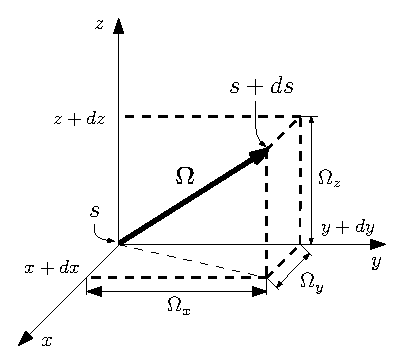
\includegraphics[width=1.15\textwidth]{obr/cartesian_streaming2}
	  \end{columns}\vspace{1em}
  \item<4-> $L\angflux \equiv \bomega\cdot\nabla\angflux + \Sigma_t\angflux = P\quad \Longrightarrow\quad \angflux = \alert<5>{L^{-1}}P$ \uncover<5->{\\(\alert<5>{umíme na charakteristikách})}
\end{itemize}

\end{frame}

\begin{frame}
  \frametitle{Integrální tvar}
  
  \begin{myitemize}
    \item Rovnice na charakteristice:~ $\der{\angflux(\br,\bomega)}{s} + \Sigma_t(\br,\bomega)\angflux(\br,\bomega) = P(\br,\bomega)$
    \item Řešení:~~ $\angflux(\br,\bomega) = \angflux(\br_0,\bomega)e^{-\tau(\br,\br_0)} + \int_0^{s_0} P(\br',\bomega)e^{-\tau(\br,\br')}\,\d{s'}$
    \begin{itemize}
    	\item $\br' = \br - s' \bomega$,~ $\br_0 = \br - s_0 \bomega$\\[.2em]
    	\item $\tau(\br,\br') = \tau(\br,\br-s'\bomega) = \int_0^{s'} \Sigma_t(\br - s''\bomega)\,\d{s''}$
    \end{itemize}
  \end{myitemize}
  \vspace{-.5em}
  \begin{center}
    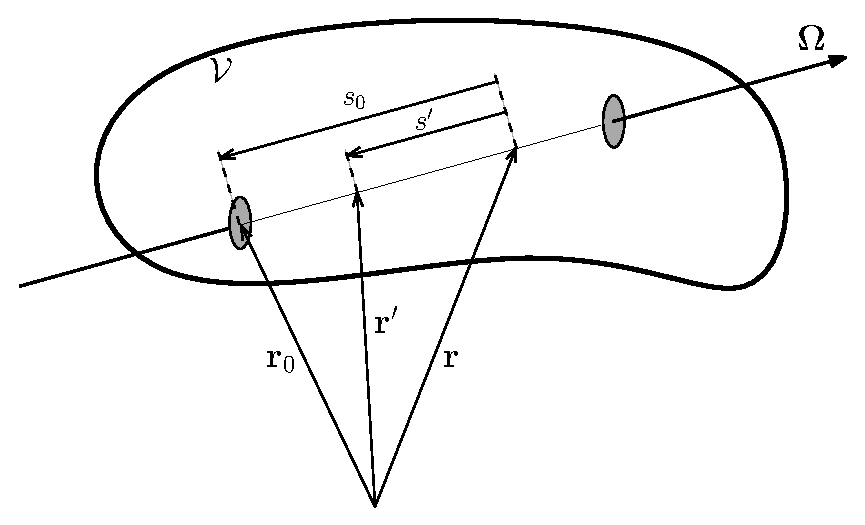
\includegraphics[scale=.5]{obr/trepka}
  \end{center}
  \vspace{-1em}
\end{frame}

\begin{frame}
  \frametitle{Integrální tvar}
  $$
    \angflux(\br,\bomega) = {\color<1>{red}\angflux(\br_0,\bomega)e^{-\tau(\br,\br_0)}} + {\color<2>{red}\int_0^{s_0} P(\br',\bomega)e^{-\tau(\br,\br')}\,\d{s'}}
  $$\\[1em]
  \ldots\ \alert<1>{neutrony, jež vstoupily do $\VV$ v $\br_0$ a dolétly do $\br$ (nebyly zachyceny)}\\
  $\hphantom{\ldots\ }$ + \alert<2>{neutrony ze zdrojů mezi $\br_0$ a $\br$, které nebyly zachyceny a dolétly do $\br$}\\
  $\hphantom{\ldots\ }$ (všechny uvažované neutrony letěly ve směru $\bomega$)
  \vspace{1em}
  \begin{itemize}[<3>]
    \item Na této formulaci jsou založeny např.
    \begin{itemize}
    	\item metoda charakteristik (MOC)
    	\item metoda kolizních pravděpodobností (CP)
    	\item nepřímo i metoda Monte Carlo (MC)
    \end{itemize}
  \end{itemize}


\end{frame}

\begin{frame}
  \frametitle{Trasování pohybu neutronů v integrálních metodách}
  \framesubtitle{Monte Carlo}
  \begin{center}
    \includegraphics<1>[scale=.5]{obr/MC}
    \includegraphics<2>[scale=.5]{obr/MC2}
  \end{center}
\end{frame}

\begin{frame}
  \frametitle{Trasování pohybu neutronů v integrálních metodách}
  \framesubtitle{Metoda (dlouhých) charakteristik}
  \vspace{-.4em}
  \begin{center}
    \includegraphics<1>[scale=.5]{obr/MOC}
    \includegraphics<2->[scale=.25]{obr/MOC2}
  \end{center}
  \only<2->{\vspace{-1.4em}}
  \begin{itemize}
    \only<1>{\item Geometrické informace (délky segmentů) lze spočíst nezávisle na $\angflux$}
  	\only<2->{\item Výpočet $\angflux_i(\bomega) = \Vint[\VV_i]{\angflux(\br,\bomega)}$ pro každou zónu nasčítáním příspěvků z jednotlivých charakteristik ve směru $\bomega$ (kvadratura pro prostor. int.)}
  	\item<3> Výpočet $\flux_i = \Vint{\flux(\br)}$ pro každou zónu nasčítáním $\angflux_i(\bomega)$ z charakteristik v jednotlivých směrech (kvadratura pro int. přes směry)
  \end{itemize}
  
\end{frame}



%    % zmínit paritní
%  \section{Matematická reprezentace rozptylu neutronů}
%    \begin{frame}[t]
  \frametitle{Geometrie rozptylu}
  \vspace{.2em}
  \begin{itemize}
  	\item Anizotropní rozptyl v \textcolor{structure}{\emph{izotropním prostředí}} je vyjádřen funkcí \alt<1>{$\chi_s$}{\alert<2>{$\Sigma_s$}}:
  	\begin{overlayarea}{\textwidth}{2.35em}
  	\shorten{-.5em}{-.5em}
  	$$
  	  \alt<1>{
  	    \chi_s(\bomega'\ra\bomega) = \chi_s(\bomega\ra\bomega') = \chi_s(\bomega'\cdot\bomega) = \chi_s(\mu_0)
  	  }{
  	    \alert<2>{\Sigma_s(\br,\bomega'\ra\bomega)} = \Sigma_s(\br,\bomega\ra\bomega') = \Sigma_s(\bomega'\cdot\bomega) = \Sigma_s(\mu_0)
  	  },
  	$$
  	\lengthen
  	\end{overlayarea}
  	kde $\mu_0 = \cos \vartheta_0$ ~(kosinus rozptylového úhlu)\\[.5em]
  	
  	\only<1>{
      \centering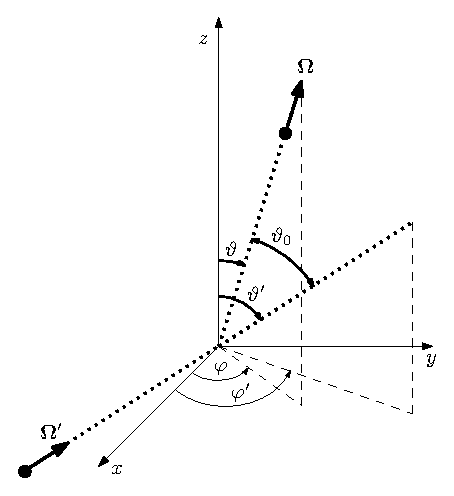
\includegraphics[scale=.75]{obr/scattering}
    }
  	\item<3->[$\Rabullet$] k popisu rozptylu nepotřebujeme zkoumat kartézský součin dvou sfér, nýbrž jen interval $[-1,1]$\\[1em]
  	\item<4-> V Hilbertově prostoru $\mathcal{H}([-1,1])$ můžeme funkci $\Sigma_s(\mu_0)$ ekvivalentně zapsat ve tvaru (zobecněného) Fourierova rozvoje vzhledem ke vhodné \alert<6>{úplné ortogonální bázi}
  	\item<5-> S jeho pomocí se budeme snažit vyjádřit \emph{\textcolor{structure}{rotačně invariantní}} operátor rozptylu $H$:
  	$$
  	  (H\angflux)(\br,\bomega) = \aintp{
        \Sigma_s(\br, \bomega'\cdot\bomega)
        \angflux(\br,\bomega')
      }
  	$$
  	ve finitní podobě (implementovatelné do počítače)
  \end{itemize}

\end{frame}

\begin{frame}
  \frametitle{Legendreovy polynomy}
  \vspace{-1em}
  \centering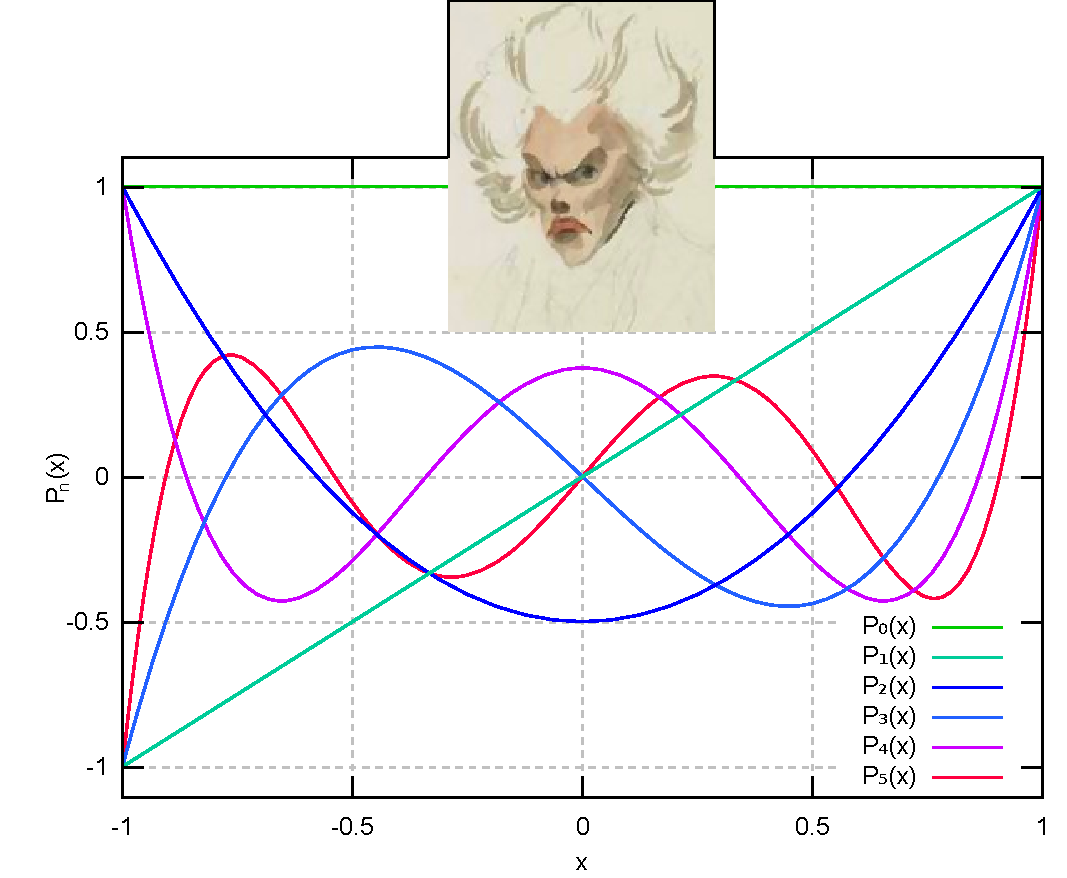
\includegraphics[height=.8\textheight]{obr/legendre}
  %\vspace{-1em}
  \begin{itemize}
  	\item \footnotesize $\P{0}(\mu) = 1,\ \ \P{1}(\mu) = \mu,\ \ \P{2}(\mu) = \frac12(3\mu^2 - 1),\ \ \P{2}(\mu) = \frac{1}{8} \left(3-30 \mu ^2+35 \mu ^4\right),\ \ \ldots$
  \end{itemize}
\end{frame}

\begin{frame}[t]
  \frametitle{Rozvoj do řady Legendreových polynomů}
  
  	  \centering$\Sigma_s(\br, \mu_0) = \suma[k]{0}{\infty}\frac{2k+1}{4\pi}\Sigma_{sk}(\br)\P{k}(\mu_0)$\\[.5em]
  	  
  \begin{itemize}	  
	  \item<2-> $\muint \P{j}(\mu)\P{k}(\mu) = \frac{2\delta_{jk}}{2k + 1}$\\[1em]
	  \item<2->[\Rabullet] $\Sigma_{sk}(\br) = 2\pi \muint[_0] \P{k}(\mu_0)\Sigma_s(\br, \mu_0)$
      \uncover<3->{\\[1em]
        $\Sigma_{s0}(\br) = \Sigma_s(\br)$\\[.5em]
   	    $\Sigma_{s1}(\br) = 2\pi \muint[_0] \mu_0\Sigma_s(\br, \mu_0)\uncover<4->{ = \muav(\br) \Sigma_s(\br)}$
   	    \begin{myitemize}
   	    	\item<4-> $ \muav(\br) = \frac{2\pi \muint[_0] \mu_0\Sigma_s(\br, \mu_0)}{2\pi \muint[_0] \Sigma_s(\br, \mu_0)} $~~\ldots~ 
   	    	\emph{střední kosinus rozptylových úhlů}\uncover<5>{\\[.5em]
   	    	$\big( = 2/(3A)$ pro elastický rozptyl na atomu s nukleonovým číslem $A\,\big)$}
   	    \end{myitemize}
   	}
  \end{itemize}

\begin{tikzpicture}[remember picture,overlay]  
  \node [xshift=-0.9cm,yshift=-1.1cm] at (current page.north east)
    {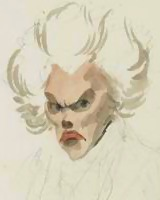
\includegraphics[width=1.5cm]{obr/Legendre.jpg}};
\end{tikzpicture}

\end{frame}

\begin{frame}
  \frametitle{Součtový vzorec}
\vspace{.75em}
\begin{overlayarea}{\textwidth}{\textheight}
\begin{itemize}
	\item Chceme vyjádřit
	  \alt<1-2>{
      $$
    	  (H\angflux)(\br,\alert<1-2>{\bomega}) = \aintp{
          \Sigma_s(\br, \bomega'\cdot\alert<1-2>{\bomega})
          \angflux(\br,\bomega')
        }
    	$$
   }{\\[1em]\hspace{1em}
      $
    	  (H\angflux)(\br,\alert<1-2>{\bomega}) = \aintp{
          \Sigma_s(\br, \bomega'\cdot\alert<1-2>{\bomega})
          \angflux(\br,\bomega')
        }
    	$
    	\vspace{0.75em}
   }
  \item<2-7> Zatím máme jen 
    \alt<1-2>{
      $$
        \Sigma_s(\br, \textcolor<2>{cyan}{\mu_0}) = \suma[k]{0}{\infty}\frac{2k+1}{4\pi}\Sigma_{sk}(\br)\P{k}(\textcolor<2>{cyan}{\mu_0})
      $$
      \vspace{-1.65em}
    }{\\[1em]\hspace{1em}
      $\Sigma_s(\br, \textcolor<2>{cyan}{\mu_0}) = \suma[k]{0}{\infty}\frac{2k+1}{4\pi}\Sigma_{sk}(\br)\P{k}(\textcolor<2>{cyan}{\mu_0})$
      \vspace{-.25em}
    }
    \alt<2-3>{
      \begin{align*}
	      \textcolor<2>{cyan}{\mu_0} &= \textcolor<2>{cyan}{\bomega'\cdot\bomega}
	      \uncover<3->{\\
      &= \lvect{\sint'\cosp',\sint'\sinp',\cost'}\!\cdot\!
	      \lvec{\sint\cosp,\sint\sinp,\cost}\\
      & = \mu'\mu + \sqrt{(1-\mu'^2)(1-\mu^2)}\cos(\azimuthal' - \azimuthal)\qquad\quad\qquad \big(\,\mu = \cos(\polar)\,\big)    
        }
      \end{align*}\vspace{-.5em}
    }{\\[1.25em] ale \vspace{-.25em}
      \begin{align*}
        \P{k}(\mu_0)
        &=P_k(\mu) P_k(\mu')+2 \sum _{m = 1}^k \frac{(k-m)!}{(k+m)!} \cos \bigl(m(\azimuthal - \azimuthal')\bigr) P_k^m(\mu) P_k^m(\mu')
        \uncover<5-7>{\\
        &=\frac{4\pi}{2k+1}\suma[m]{-k}{k}\textcolor<7>{blue}{\Y{k}{m}}(\alt<5>{\polar,\azimuthal}{\alert<6>{\bomega}})\textcolor<7>{blue}{\Yc{k}{m}}(\alt<5>{\polar',\azimuthal'}{\alert<6>{\bomega'}})
        }
      \end{align*}
    }
\end{itemize}
\end{overlayarea}

\begin{tikzpicture}[remember picture,overlay]  
  \alt<1-2>{
    \node [xshift=-0.9cm,yshift=-1.1cm] at (current page.north east)
      {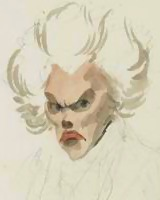
\includegraphics[width=1.5cm]{obr/Legendre.jpg}};
  }{
    \node [xshift=-2.7cm,yshift=-3cm] at (current page.north east)
      {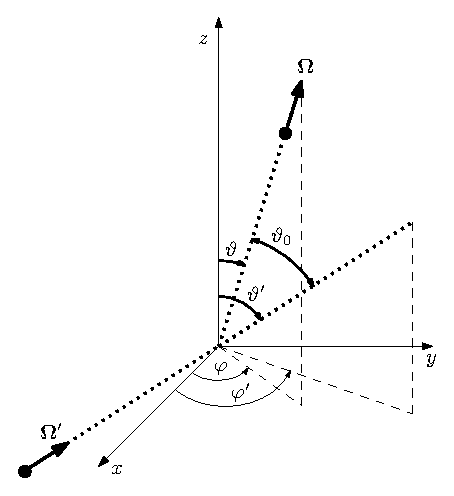
\includegraphics[width=5cm]{obr/scattering}};
  }
  \only<3->{
    \node [xshift=0.9cm,yshift=1.1cm] at (current page.south west)
      {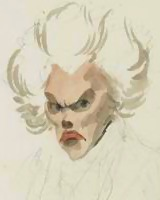
\includegraphics[width=1.5cm]{obr/Legendre.jpg}};
  }
\end{tikzpicture}

\end{frame}

\begin{frame}
  \frametitle{Sférické harmoniky}
  \framesubtitle{Definice}
  \begin{itemize}
  	\item<1-3> Sférická harmonická funkce \textcolor{structure}{\emph{řádu $m$}} a \textcolor{structure}{\emph{stupně $l$}}
  	  \begin{gather*}
        \Y{l}{m}(\bomega) = \Y{l}{m}(\alt<1>{\polar}{\mu},\azimuthal) = \sqrt{\frac{2l+1}{4\pi}\frac{(l-m)!}{(l+m)!}} \P{l}^m(
          \alt<1>{\cos\polar}{\mu}
        )e^{i m \azimuthal}\\[.5em]
        \alt<1>{\polar\in [0,\pi]}{\mu\in[-1,1]},\ \azimuthal\in [0,2\pi),\quad 
        l\in\mathbb{N}_0,\ m\in\mathbb{Z},\ 0\leq m \leq l
      \end{gather*}
    \item<3> \textcolor{structure}{\emph{Přidružené Legendreovy funkce}} (\emph{Associated Legendre functions})
    $$
      \P{l}^m(\mu) = 
      \begin{cases} 
        (-1)^m\sqrt{(1-\mu^2)^m}\ \der[m]{\P{l}(\mu)}{\mu} & \hphantom{-}\,0 \leq m \leq l,\\[1em]
        \displaystyle (-1)^{-m}\,\frac{(l+m)!}{(l-m)!}\P{l}^{-m}(\mu) & -l \leq m < 0 
      \end{cases}
    $$
  \end{itemize}
  
\begin{tikzpicture}[remember picture,overlay]  
  \node [xshift=-1cm,yshift=-0.8cm] at (current page.north east)
    {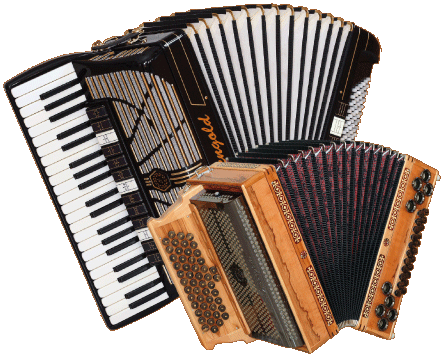
\includegraphics[width=1.75cm]{obr/harmoniky.png}};

   \only<4>{ 
     \node [anchor=center,yshift=-0.8cm] at (current page.center)
       {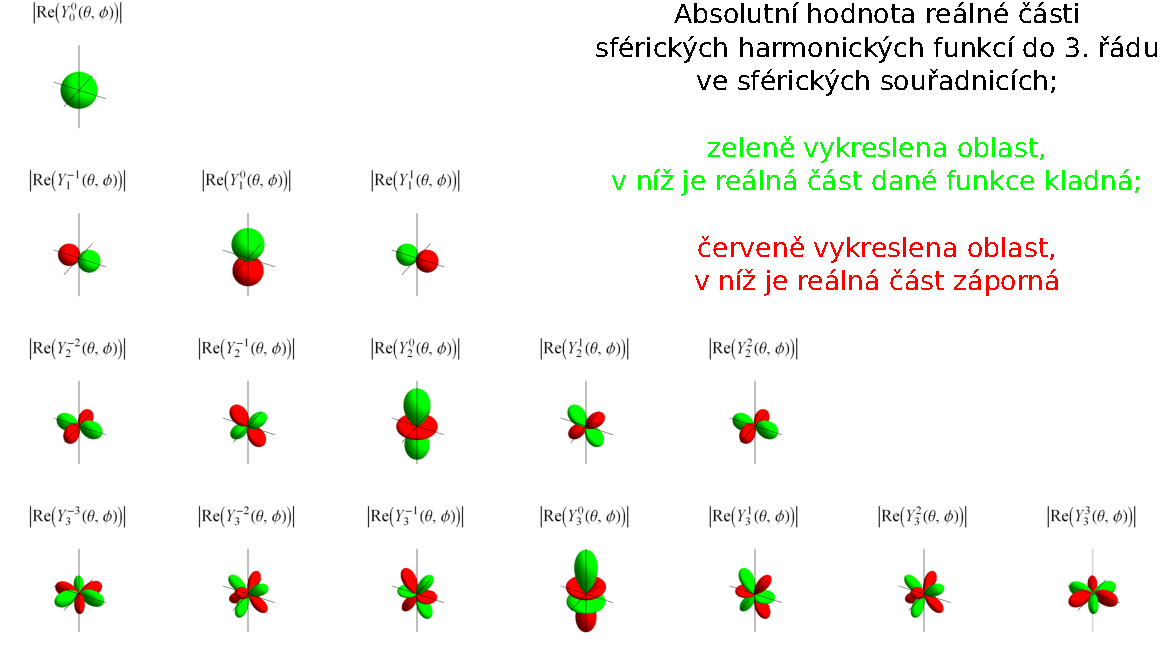
\includegraphics[width=1.05\textwidth]{obr/sh}};
   }
\end{tikzpicture}

\end{frame}

\begin{frame}
  \frametitle{Sférické harmonické funkce}
  \framesubtitle{Vlastnosti}
  \begin{itemize}
  	\item Úplný ortonormální systém na sféře vzhledem ke skalárnímu součinu
  	  $$
        \aint{\Y{l}{m}(\bomega)\Yc{l}{m}(\bomega)}
        = \int_{0}^{2\pi}\d{\azimuthal}\int_{-1}^{1}\d{\mu}
        \Y{l}{m}(\mu,\azimuthal)\Yc{l'}{m'}(\mu,\azimuthal)
      $$
    \item SHF stupně $l$ generují rotačně invariantní podprostor $\Lp{2}(\SS)$:
      $$\Lambda_l = \mathrm{Span}\bigl\{\Y{l}{m}; -l \leq m \leq l\bigr\},$$
    takový, že $R(\Lambda_l) \subset \Lambda_l$ pro libovolnou rotaci $R$
    \begin{itemize}
    	\item<2-> vlastní prostor příslušný $l$-tému vl. č. Laplaceova-Beltramiho
    operátoru $\nabla\cdot(\nabla)$ na sféře
      \item<3-> \alert{vlastní prostor libovolného rotačně invariantního operátoru}
    \end{itemize}
    
    \item<4-> Lze je použít pro zobecněný Fourierův rozvoj (tzv. \emph{Laplaceův rozvoj})
    funkcí def. na sféře -- 3D analogie rozvoje pomocí trigon. polynomů
    \item<5-> Azimutálně symetrické (nezávislé na $\azimuthal$ SHF: Legendreovy polynomy
   
  \end{itemize}
\end{frame}

\begin{frame}
  \frametitle{Sférické harmonické funkce}
  \framesubtitle{Použití -- reprezentace operátoru rozptylu}
  
  \begin{itemize}
  	\item Zobecněný Fourierův rozvoj rotačně invariantního operátoru rozptylu
  	do řady jeho vlastních funkcí
  \end{itemize}
\begin{align*}
\alert<6>{(H\angflux)(\br,\bomega)} &= 
  \aintp{
    \Sigma_s(\br, \bomega'\cdot\bomega)
    \angflux(\br,\bomega')
  }\uncover<2->{\\
& = \aintp{
      \suma[k]{0}{\infty}
        \frac{2k+1}{4\pi}\Sigma_{sk}(\br)\P{k}(\bomega'\cdot\bomega)
        \angflux(\br,\bomega')
    }\uncover<3->{\\
& = \aintp{
      \suma[k]{0}{\infty}
	      \Sigma_{sk}(\br)\suma[m]{-k}{k}\Y{k}{m}(\bomega)\Yc{k}{m}(\bomega')
        \angflux(\br,\bomega')
    }\uncover<4->{\\
& = \suma[k]{0}{\infty}
	    \Sigma_{sk}(\br)\suma[m]{-k}{k}\Y{k}{m}(\bomega) \aintp{
	      \Yc{k}{m}(\bomega')\angflux(\br,\bomega')
	    }\uncover<5->{\\
& \alert<6>{= \suma[k]{0}{\infty}
      \Sigma_{sk}(\br)\suma[m]{-k}{k}\Y{k}{m}(\bomega)\angmomgen{k}{m}(\br)}
}}}}
\end{align*}

\end{frame}

\begin{frame}
  \frametitle{Sférické harmonické funkce}
  \framesubtitle{Použití -- reprezentace operátoru rozptylu}
  
  \centering \alert<1>{$(H\angflux)(\br,\bomega) = \suma[k]{0}{\infty}\Sigma_{sk}(\br)\suma[m]{-k}{k}\Y{k}{m}(\bomega)\alert<2>{\angmomgen{k}{m}(\br)}$}
  
  \begin{itemize}
  	\item<2-> \alert<2>{$\angmomgen{k}{m}(\br) = \aint{\Yc{k}{m}(\bomega)\angflux(\br,\bomega)}$}\vspace{.5em}
  	\begin{itemize}
  		\item[\ldots]	  koeficienty zobecněného Fourierova rozvoje $\angflux(\br,\bomega)$ vzhledem k $\bomega$:
  		  \vspace{-.5em}
    		  \begin{equation*}
    		    \angflux(\br,\bomega) = \suma[k]{0}{\infty}\suma[m]{-k}{k}\angmomgen{k}{m}(\br)\Y{k}{m}(\bomega)
    		  \end{equation*}
   	\end{itemize}
    \item<3-> Finitní reprezentaci operátoru rozptylu získáme použitím konečného rozvoje ($0 \leq k \leq L < \infty$):
    \begin{myitemize}
    	\item rozptylovací charakteristiku každého materiálu uchováváme v podobě pole příslušných koeficientů $\Sigma_{sk}$
    \end{myitemize}
  \end{itemize}

\end{frame}

\begin{frame}
  \frametitle{Sférické harmonické funkce}
  \framesubtitle{Použití -- metoda $P_L$}
  
  \begin{itemize}
  	\item  Rozvoj 
  	  \begin{equation*}
		    \angflux(\br,\bomega) = \suma[k]{0}{L}\suma[m]{-k}{k}\angmomgen{k}{m}(\br)\Y{k}{m}(\bomega)
		  \end{equation*}
		  pro $L < \infty$ lze použít přímo k definici přibližného řešení LBR:
		  \begin{myitemize}
		  	\item dosazením rozvoje do LBR, použitím rozvoje operátoru rozptylu z předchozích slajdů a 
		  	  aplikací Galerkinovy metody vzhledem ke směrové proměnné získáme soustavu PDR 1. řádu 
		  	  v prostorové proměnné
		  	\item řešením vzniklé úlohy obdržíme $\angmomgen{k}{m}(\br)$, a tedy i $\angflux(\br,\bomega)$
		  \end{myitemize}
  \end{itemize}
  \uncover<2>{
\vspace{1em}
  \begin{center}
    {\huge  \textcolor{blue}{\emph{ O tom ale zas až někdy příště ...} ;-)}}
  \end{center}
  }
\end{frame}

%    
%
%\part{Monoenergetická transportní rovnice v 1D}
%
%  \section{Rovnice "doleva/doprava"}
%    \begin{frame}
  \frametitle{Transport neutronů ve dvou směrech}
  
  \begin{myitemize}
    \item Monoenergetický, ustálený stav, pro jednoduchost bez štěpení
    \begin{itemize}
    	\item $\Sigma_t = \Sigma_a + \Sigma_s$
    \end{itemize}
	  \item Pohyb neutronů omezen do dvou směrů:
	  $$
	    \bomega \equiv \bomega_x \equiv \mu = 
	    \begin{cases}
	      +1 & \quad \mbox{(kladná poloosa $x$)},\\
	      -1 & \quad \mbox{(záporná poloosa $x$)}
	    \end{cases}
	  $$
	  \item<2-> $\angflux_{\pm}(x) = \angflux(x,\pm 1)$
	  \item<2-> $\flux(x) = \angflux_+(x) + \angflux_-(x)$
	  \item<2-> $J(x) = (+1)\angflux_+(x) + (-1)\angflux_-(x) = \angflux_+(x) - \angflux_-(x)$
	  \item<2-> $Q_\pm = Q(x,\pm 1)$
  \end{myitemize}

\end{frame}

\begin{frame}
  \frametitle{Transport neutronů ve dvou směrech}
  \framesubtitle{Rozptyl}
    \vspace{-1em}
	  \begin{gather*}
      \Sigma_s(x,\mu'\ra\mu) = 
      \begin{cases}
        \Sgmr(x) & \ \; \mu'\mu = +1,\\
        \Sgml(x) & \ \; \mu'\mu = -1,
      \end{cases}\\[.5em]
	    \Sigma_s(x) = \Sgml(x) + \Sgmr(x)
    \end{gather*}

    \begin{itemize}
    	\item střední hodnota kosinu rozptylového úhlu:
    	$$
    	  \muav = \frac{(+1)\Sgmr + (-1)\Sgml}{\Sgmr + \Sgml} = \frac{\Sgmr - \Sgml}{\Sigma_s}
    	$$
    	\item<2-> izotropní rozptyl: $$\Sgmr = \Sgml = \frac{\Sigma_s}{2}\quad \Longrightarrow\quad \muav = 0$$
    	\item<2-> bez rozptylu (neutrony nemění při kolizích směr):
          	$$\Sigma_s = \Sgmr \quad \Longrightarrow\quad \muav = 1$$
    \end{itemize}

\end{frame}

\begin{frame}
  \frametitle{Lineární Boltzmannova rovnice v dvousměrovém modelu}

    $$
      \pm\der{\angflux_{\pm}(x)}{x} + \Sigma_t(x)\angflux_{\pm}(x) = 
      \Sgmr(x)\angflux_{\pm}(x) + \Sgmr(l)\angflux_{\mp}(x) + Q_{\pm}(x)
    $$
    

    \begin{itemize}
    	\item<2-> sečtením obou rovnic ~~~ (označ. $Q = Q_+ + Q_-$):
    	$$
    	  \der{J}{x} + \Sigma_t\flux = \Sigma_s\flux + Q
    	  \quad\Longrightarrow\quad
    	  \der{J}{x} + \Sigma_a\flux = Q
    	$$
    	\item<3-> odečtením obou rovnic ~ (označ. $J_Q = Q_+ - Q_-$):
    	$$
    	  \der{\flux}{x} + \Sigma_t J = \muav\Sigma_s J + J_Q
    	  \quad\Longrightarrow\quad
    	  J = -\frac{1}{\Sigma_t-\muav\Sigma_s}\left(\der{\flux}{x} - J_Q\right)
    	$$
    	\item<4->[$\Rightarrow$] S využitím standardních definic \alert<5>{klasické difúzní teorie}:
    	$$
    	  D = \frac{1}{\only<5>{\alert3}\Sigma_{tr}} = \frac{1}{\only<5>{\alert{3(}}\Sigma_t-\muav\Sigma_s\only<5>{\alert)}}
    	$$
    	nakonec dostaneme LBR ve tvaru
    	$$
    	  -\der{}{x}\bigg[D(x)\der{\flux(x)}{x}\bigg] + \Sigma_a(x)\flux(x) = Q(x) - \der{}{x}\bigg[D(x)J_Q(x)\bigg]
    	$$
    	\end{itemize}

\end{frame}

\begin{frame}
  \frametitle{Lineární Boltzmannova rovnice v dvousměrovém modelu}
  \framesubtitle{Doplňující podmínky a vztahy}
    \vspace{.75em}\centering $\VV = (x_{b-}\;,\; x_i)\; \cup\; (x_i\; ,\; x_{b+})$\\[.25em]
    \begin{itemize}
    	\item Okrajová podmínka na volné hranici:
        $$
        \angflux_\mp(x_{b\pm}) = 0\quad \Longrightarrow\quad \mp D\left.\der{\flux}{x}\right\vert_{x_{b\pm}} = \left.\vphantom{\der{\flux}{x}}\big(\flux \mp D J_Q\big)\right\vert_{x_{b\pm}}
    		$$
    	\item Podmínky na vnitřních rozhraních:
    	\begin{myitemize}
    		\item $0 = \Delta(\angflux) := \lim\limits_{x\to x_i+}\angflux_\pm(x) - \lim\limits_{x\to x_i-}\angflux_\pm(x)$
    		\item $\Delta\bigg(D\der{\flux}{x}\bigg) = \Delta(D J_Q)$
    	\end{myitemize}\vspace{.5em}
    	\item Vztah mezi směrovými toky skalárním tokem:
    	$$
  	    \angflux_\pm(x) = \frac12\bigg[\flux(x) \pm J(x)\bigg] = \frac12\bigg[\flux(x)\mp D(x)\der{\flux(x)}{x} \pm D(x)J_Q(x)\bigg]
    	$$  	
    \end{itemize}

\end{frame}

\begin{frame}
  \frametitle{Lineární Boltzmannova rovnice v dvousměrovém modelu}
  \framesubtitle{Difúzní podoba}
      
      \textcolor{structure}{\emph{Pro izotropní zdroje}} ($J_Q = 0$) máme formálně \alert<2>{klasickou rovnici difúze neutronů} v samoadjungovaném tvaru
    	$$
    	  -\der{}{x}\bigg[D(x)\der{\flux(x)}{x}\bigg] + \Sigma_a(x)\flux(x) = Q(x)
    	$$
    	s extrapolovanou okrajovou podmínkou na volné hranici:
    	$$
      	\mp \left.\frac{1}{\flux}\der{\flux}{x}\right\vert_{x_{b\pm}} = \frac{1}{\only<2->{\alert{2}}D(x_{b\pm})} = \only<2->{\alert{\frac32}}\Sigma_{tr}(x_{b\pm})
    	$$
    	a spojitostí proudů a toků na vnitřních rozhraních
    	
\end{frame}

\begin{frame}
  \frametitle{Příklad 1 -- v prostoru rozložený izotropní zdroj}
  \framesubtitle{Data}
  
  \centering$a = 5$\,cm\\[1em]
  \centering$\VV = \textcolor{matCdk}{(-\infty, -a)} \; \cup \; \textcolor{matBdk}{(-a,a)} \; \cup \; \textcolor{matCdk}{(a,+\infty)}$

\begin{center}
	\begin{tabular}{|ABC|}
	  \hline
		 & $\abs{x} < a$ & $\abs{x} > a$ \nl
		$\Sigma_t\,[\mathrm{cm}^{-1}]$ & 1.00 & 0.50 \nl
		$\Sigma_a\,[\mathrm{cm}^{-1}]$ & 0.55 & 0.10 \nl
		$Q\,[\mathrm{cm}^{-1}s^{-1}]$ & 0.10 & 0.00 \nl
		$\muav$ & $\textcolor<2>{blue}{\bar\mu_{01}}$ & $\textcolor<2>{blue}{\bar\mu_{02}}$
		\nl
	\end{tabular}
\end{center}

\end{frame}

\begin{frame}
  \frametitle{Příklad 1 -- v prostoru rozložený izotropní zdroj}
  \framesubtitle{$\bar\mu_{01} = 0.75$~~~~$\bar\mu_{02} = 0.5$}
  
	\centering\includegraphics[height=.8\paperheight]{obr/doleva_doprava/distribuovany_075_05}

\end{frame}

\begin{frame}
  \frametitle{Příklad 1 -- v prostoru rozložený izotropní zdroj}
  \framesubtitle{$\bar\mu_{01} = 0$ (izotropní rozptyl)~~~~$\bar\mu_{02} = 0.5$}
  
  \centering\includegraphics[height=.8\paperheight]{obr/doleva_doprava/distribuovany_0_05}

\end{frame}

\begin{frame}
  \frametitle{Příklad 1 -- v prostoru rozložený izotropní zdroj}
  \framesubtitle{$\bar\mu_{01} = 1$ (bez rozptylu)~~~~$\bar\mu_{02} = 0.5$}
  
  \centering\includegraphics[height=.8\paperheight]{obr/doleva_doprava/distribuovany_1_05}

\end{frame}

\begin{frame}
  \frametitle{Příklad 1 -- v prostoru rozložený izotropní zdroj}
  \framesubtitle{$\bar\mu_{01} = 0.75$~~~~$\bar\mu_{02} = 1$ (bez rozptylu)}
  
  \centering\includegraphics[height=.8\paperheight]{obr/doleva_doprava/distribuovany_075_1}

\end{frame}

\begin{frame}
  \frametitle{Příklad 1 -- v prostoru rozložený izotropní zdroj}
  \framesubtitle{$\bar\mu_{01} = 1$ (bez rozptylu)~~~~$\bar\mu_{02} = 1$ (bez rozptylu)}
  
  \centering\includegraphics[height=.8\paperheight]{obr/doleva_doprava/distribuovany_1_1}

\end{frame}

\begin{frame}
  \frametitle{Příklad 2 -- bodový anizotropní zdroj}
  \framesubtitle{Data}
  
  \centering $\VV = (0,a)$~ ve vakuu\\
  
  \begin{myitemize}
  	\item $a = 5$\,cm
  	\item $\Sigma_t = 1$\,cm$^{-1}$,~ $\Sigma_a = 0.5$\,cm$^{-1}$
  	\item $S_+ = 0.7$\,s$^{-1}$,~ $S_- = 0.3$\,s$^{-1}$\\[.5em]
  	      $Q_\pm(x) = S_\pm\delta(x-x_Q)$ [cm$^{-1}$s$^{-1}$]\\[.5em]
  	      $x_Q=2$\,cm
  	\item $\muav = \textcolor<2>{blue}{\bar\mu_{01}}$
  \end{myitemize}


\end{frame}

\begin{frame}
  \frametitle{Příklad 2 -- bodový anizotropní zdroj}
  \framesubtitle{$\bar\mu_{01} = 0.75$}
  
  \centering\includegraphics[height=.75\paperheight]{obr/doleva_doprava/bodovy_075}

\end{frame}

\begin{frame}
  \frametitle{Příklad 2 -- bodový anizotropní zdroj}
  \framesubtitle{$\bar\mu_{01} = 0$ (izotropní rozptyl)}
  
  \centering\includegraphics[height=.75\paperheight]{obr/doleva_doprava/bodovy_0}

\end{frame}

\begin{frame}
  \frametitle{Příklad 2 -- bodový anizotropní zdroj}
  \framesubtitle{$\bar\mu_{01} = 1$ (bez rozptylu)}
  
  \centering\includegraphics[height=.75\paperheight]{obr/doleva_doprava/bodovy_1}

\end{frame}

%\begin{frame}
%  \frametitle{Příklad -- v prostoru rozložený anizotropní zdroj}
%  \framesubtitle{Popis a tvar řešení}
%
%
%\end{frame}
%
%\begin{frame}
%  \frametitle{Příklad -- v prostoru rozložený anizotropní zdroj}
%  \framesubtitle{Průběh neutronových toků}
%
%
%\end{frame}

%  \section{Směrová závislost s azimutální symetrií}
%    \begin{frame}
  \frametitle{Bilance směrového toku v azimutálně symetrickém případě}
  \framesubtitle{Transport}


\end{frame}

\begin{frame}
  \frametitle{Bilance směrového toku v azimutálně symetrickém případě}
  \framesubtitle{Rozptyl}


\end{frame}

\begin{frame}
  \frametitle{Bilance směrového toku v azimutálně symetrickém případě}
  \framesubtitle{Zdroje}


\end{frame}

\begin{frame}
  \frametitle{Bilance směrového toku v azimutálně symetrickém případě}
  % + O. P.

\end{frame}



%  \subsection{Metoda $P_N$}
%    \begin{frame}
  \frametitle{$P_N$ aproximace}
  \framesubtitle{Základní princip}  


\end{frame}

\begin{frame}
  \frametitle{$P_N$ aproximace}
  \framesubtitle{Obecný tvar rovnic}  


\end{frame}

\begin{frame}
  \frametitle{$P_N$ aproximace}
  \framesubtitle{Okrajové podmínky}  


\end{frame}

\begin{frame}
  \frametitle{$P_N$ aproximace}
  \framesubtitle{Speciální případy}  


\end{frame}

\begin{frame}
  \frametitle{Přechod k difúzní aproximaci}


\end{frame}

\begin{frame}
  \frametitle{Difúzní tvar $P_N$ rovnic vyššího řádu}


\end{frame}


%  \subsection{Metoda $S_N$}
%    \begin{frame}
  \frametitle{$S_N$ aproximace}
  \framesubtitle{Základní princip}  


\end{frame}

\begin{frame}
  \frametitle{$S_N$ aproximace}
  \framesubtitle{Gaussova-Legendreova kvadratura}  


\end{frame}

\begin{frame}
  \frametitle{$S_N-P_{N-1}$ aproximace}
  \framesubtitle{Obecný tvar rovnic}  


\end{frame}

\begin{frame}
  \frametitle{$S_N-P_{N-1}$ aproximace}
  \framesubtitle{Okrajové podmínky}  


\end{frame}

%
%  \section{Iterační řešení}
%    \begin{frame}
  \frametitle{Diskretizace prostorové závislosti}
  


\end{frame}

\begin{frame}
  \frametitle{Iterační řešení}
  


\end{frame}

\begin{frame}
  \frametitle{Příklad}
  


\end{frame}

\begin{frame}
  \frametitle{Provázání směrové a prostorové diskretizace}
  


\end{frame}

\begin{frame}
  \frametitle{Příklad}
  


\end{frame}

%
%\part{Reálné úlohy -- metody řešení 3D transportní rovnice}
%
%  \section{Potíže s metodami $P_N$, $S_N$ ve více dimenzích}
%  \section{Metoda $SP_N$}

%\section{Monoenergetická transportní rce. ve více dimenzích}

%\subsection{Sférické harmonické funkce}
%\subsection{Potíže s metodami $P_N$, $S_N$}
%\subsection{Metoda $SP_N$}
%\subsubsection{Formální odvození}
%\subsubsection{Teoretické vlastnosti}
%\subsubsection{Numerická ukázka}

%\section{Aproximace energetické závislosti}

\begin{frame}[label=slide17]
  \frametitle<presentation>{Literatura}
  
	
  \begin{thebibliography}{\textwidth}       
  \beamertemplatearticlebibitems
	\footnotesize
	\bibitem[Ch]{Chao}
  {J. E. Hoogenboom}
	\newblock {T}HE TWO-DIRECTION NEUTRAL-PARTICLE TRANSPORT MODEL: A USEFUL TOOL FOR RESEARCH AND EDUCATION
	\newblock {\em {T}ransport {T}heory and {S}tatistical {P}hysics}, 37:65--108, 2008.

	\bibitem[FC]{Fu}
	{W. M. Stacey}
	\newblock Nuclear Reactor Physics (Chap. 9).
	\newblock {\em John Wiley \& Sons, Inc., New York}, 
	  2001.

	\bibitem[Wag]{Wagner}
	{P}. {R}euss
	\newblock {N}eutron {P}hysics
	\newblock {\em EDP Sciences}, 2008.
	
	\bibitem[DTL]{Dautray}
	{R. Dautray and J.-L. Lions}
	\newblock{Mathematical Analysis and Numerical Methods for Science and Technology:
  	6 -- Evolution Problems II (\S 6)}
  \newblock{\em Springer}, 2000.
	
	\bibitem[SAN]{Sansone}
		{G. Sansone}
	\newblock{Orthogonal Functions (Chap. 3)}
  \newblock{\em Dover Publications}, 2004.
	\end{thebibliography}
	
\end{frame}

\end{document}
